\documentclass[10pt]{report}
\usepackage[utf8]{inputenc}
\usepackage[italian]{babel}
\usepackage{multicol}
\usepackage[a4paper, total={18cm, 25cm}]{geometry}
\usepackage{graphicx}
\usepackage{xcolor}
\usepackage{textcomp}
\graphicspath{ {./img/} }
\usepackage{listings}
\lstdefinestyle{customasm}{
  belowcaptionskip=1\baselineskip,
  frame=line,
  xleftmargin=\parindent,
  language=[x86masm]Assembler,
  basicstyle=\ttfamily,
  commentstyle=\itshape\color{purple!40!black},
}
\lstset{escapechar=@,style=customasm}
\lstnewenvironment{C}
  {\lstset{language=C++,frame=none}}
  {}
\begin{document}
\title{Architettura degli Elaboratori}
\author{Appunti: Simone Pepi\\Stesura in \LaTeX: Federico Matteoni}
\date{ }
\renewcommand*\contentsname{Indice}

\maketitle
\begin{multicols}{2}
\tableofcontents
\end{multicols}
\pagebreak
\section{Introduzione}
Appunti del corso di \textbf{Architettura degli Elaboratori} presi a lezione da \textbf{Federico Matteoni}.\\\\
Prof.: \textbf{Maurizio Bonuccelli}, maurizio.angelo.bonuccelli@unipi.it\\
\begin{list}{-}{Riferimenti web:}
\item \emph{http://pages.di.unipi.it/bonuccelli/aeb.html}
\item \emph{didawiki.cli.di.unipi.it/doku.php/informatica/ae/start}
\end{list}
Ricevimento: Martedì 10-12, stanza 294 DE\\
Esame: \textbf{scritto} (\textit{closed book}) e \textbf{orale}. I compitini sono validi solo per la sessione invernale (gen-feb)\\
\begin{list}{-}{Libri}
\item  M. Vanneschi \textit{Architettura degli Elaboratori}, Pisa UniversitY Press
\item D. A. Patterson \textit{Computer Organization \& Design - The Hardware/Software Interface}
\end{list}
\section{Cosa riguarda il corso}
Consiste in come sono fatti pc internamento da un punto di vista di sottosistemi senza scendere nei dettagli elettrici.
\begin{list}{-}{Il corso è diviso in quattro parti:}
\item Fondamenti e strutturazione firmware (I Compitino)
\item Macchina assembler (D-RISC) e processi
\item Architetture General-Purpose
\item Architetture parallele (II Compitino)
\end{list}
\chapter{Fondamenti di strutturazione}
\section{Struttura a livelli}
\paragraph{Dividere} Per dedicarci allo studio di un sistema complesso spesso è utile \textbf{dividerlo in pezzi}. Nel caso di un sistema di elaborazione, in alcuni casi è \textbf{interessante avere una visione vicina alla struttura fisica} in termini di componenti hardware. In altri casi è \textbf{interessante avere una visione astratta del sistema} per poterne osservare le funzionalità e le strutture più adatte alla specifica applicazione.
\paragraph{Astrarre} Da questa necessità deriva la possibilità di strutturare un sistema a vari \textbf{livelli di astrazione} che non descrivono una reale struttura fisica, ma è \textbf{utile per ragioni specifiche} quali:
\begin{list}{}{}
\item Saper riconoscere \textbf{quale metodo di progettazione strutturata} viene seguito o conviene seguire (\textbf{top-down}, \textbf{bottom-up}, \textbf{middle-out})
\item Saper riconoscere \textbf{se i vari livelli rispettano una relazione gerarchica} oppure se non esiste alcun tipo di ordinamento
\item Essere in grado di \textbf{valutare a quali livelli conviene descrivere e implementare} determinate funzioni del sistema
\end{list}
\section{Macchine Virtuali}
\paragraph{Sistema di elaborazione} \textbf{Le funzionalità di un sistema di elaborazione} nel suo complesso possono essere \textbf{ripartite su un certo numero di livelli} che vengono definite \textbf{macchine virtuali}. \begin{list}{-}{La suddivisione può seguire \textbf{due approcci} fondamentali:}
	\item \textbf{Linguistico}: stabilisce i livelli in base ai linguaggi usati
	\item \textbf{Funzionale}: stabilisce i livelli in base a cosa fanno
\end{list}
I vari livelli sono schematizzati come in figura:
\begin{center}
\rule{5cm}{1pt} Interfaccia \rule{5cm}{1pt}\\
MV$_{i}$	R$_{i}$ = {risorse} + L$_{i}$ = {linguaggi}\\
\rule{5cm}{1pt} Interfaccia \rule{5cm}{1pt}\\
MV$_{i-1}$	R$_{i-1}$ = {risorse} + L$_{i-1}$ = {linguaggi}\\
\rule{5cm}{1pt} Interfaccia \rule{5cm}{1pt}\\
\end{center}
MV$_{i}$ realizza politica P$_{i}$ con linguaggio L$_{i}$ e risorse R$_{i}$.\\
MV$_{i}$ utilizza le funzionalità che il livello MV$_{i-1}$ (cioè le sue primitive) fornisce \textbf{attraverso l'interfaccia}.\\
L'interfaccia definita è fondamentale per poter rendere possibile la collaborazione tra le macchine virtuali, e permettere così ai linguaggi di MV$_{i}$ di sfruttare funzionalità e meccanismi di MV$_{i-1}$.\\
Le macchine virtuali godono delle \textbf{seguenti proprietà}:
\begin{list}{}{}
	\item L'\textbf{insieme} degli oggetti o risorse \textbf{R}$_{i}$ di MV$_{i}$ \textbf{è accessibile soltanto da parte dei meccanismi di L}$_{i}$ 
	\item Al livello MV$_{i}$ \textbf{non sono note le politiche adottate dai livelli inferiori}
\end{list}
\paragraph{Supporto a tempo di esecuzione} Anche detto \textbf{Runtime Support}, è l'\textbf{insieme dei livelli sottostanti}.\\
Nell'esempio, MV$_{i}$ ha come runtime support i livelli MV$_{i-1}$ \ldots MV$_{0}$.
\paragraph{Virtualizzazione ed Emulazione} Con \textbf{virtualizzazione} o astrazione intendiamo il \textbf{processo secondo cui un livello MV$_{i}$ usa funzionalità dei livelli superiori}.\\
Con \textbf{emulazione} o concretizzazione intendiamo il \textbf{processo secondo cui un livello MV$_{i}$ usa funzionalità dei livelli inferiori}.
\paragraph{Modularità} Tutte queste funzionalità sono \textbf{alla base della strutturazione di sistemi con elevata modularià}, \textbf{modificabilità}, \textbf{portabilità}, \textbf{manutebilità} e \textbf{testabilità}.
\subsection{Le Macchine Virtuali}
\begin{list}{}{}
\item \textbf{MV$_{4}$} Applicazioni\\L$_{4}$: Java, C, ML\ldots\\R$_{4}$: oggetti astratti, costrutti, tipi di dato definibili dall'utente
\item \rule{5cm}{1pt} \textit{Interfaccia}: chiamate di sistema \rule{5cm}{1pt}
\item \textbf{MV$_{3}$} Sistema Operativo\\L$_{3}$: C, linguaggi di programmazione concorrente, linguaggi sequenziali con librerie che implementano meccanismi di concorrenza\\R$_{3}$: variabili condivise, risorse condivise, oggetti astratti usati per la cooperazione tra processi e thread
\item \rule{5cm}{1pt} \textit{Interfaccia}: istruzioni assembler \rule{5cm}{1pt}
\item \textbf{MV$_{2}$} Macchina assembler\\L$_{2}$: assembler (D-RISC)\\R$_{2}$: registri, memoria, canali di comunicazione
\item \rule{5cm}{1pt} \textit{Interfaccia}: istruzioni firmware per l'assembler \rule{2.8cm}{1pt}
\item \textbf{MV$_{1}$} Firmware\\L$_{1}$: microlinguaggio\\R$_{1}$: sommatore, commutatore, registri, strutture di interconnessione intra-unità e inter-unità
\item \rule{5cm}{1pt} \textit{Interfaccia}: hardware \rule{6.7cm}{1pt}
\item \textbf{MV$_{0}$} Hardware\\L$_{0}$: \textit{funzionamento dei circuiti elettronici}\\R$_{0}$: circuiti elettronici elementari (AND, OR, NOT), collegamenti fisici, reti logiche
\end{list}
Il corso riguarderà principalmente i livelli MV$_{2}$ $\rightarrow$ MV$_{0}$ inclusi, comprese le istruzioni assembler.\\
Il livello firmware sarà fatto da \textbf{memoria}, \textbf{processore} e \textbf{dispositivi I/O}. I dispositivi di I/O comunicano bilateralmente con la memoria e il processore comunica bilateralmente con memoria. Opzionalmente, i dispositivi di I/O comunicano bilateralmente direttamente con il processore. Questa è l'\textbf{architettura standard}, presentata in maniera \textbf{estremamente semplicistica}.\\
Vedremo nel dettaglio il processore e la memoria, non i dispositivi di I/O perché troppo complessi.
\pagebreak
\subsection{Struttura Interna}
\paragraph{Da Verticale a Orizzontale} Fin'ora abbiamo parlato delle macchine virtuali in senso \textbf{verticale}, adesso vogliamo trovare un modo concettualmente uniforme -- \textbf{orizzontale} -- per poter studaire i livelli \textbf{al loro interno}.
\paragraph{Sistema di Elaborazione} Una volta scelta la struttura verticale di un sistema, dobbiamo capire come funziona l'interno di ciascun livello per poter far funzionare tutto il sistema, cioè dobbiamo capire \textbf{come funziona il sistema di elaborazione di un livello} composto da due componenti:
\begin{list}{}{}
	\item \textbf{Moduli di Elaborazione}, \textbf{ad ognuno} dei quali \textbf{è affidata l'elaborazione di un sottoinsieme di operazioni} del livello.
	\item \textbf{Struttura di Interconnessione}, \textbf{con la quale i moduli} di elaborazione del livello \textbf{cooperano e comunicano tra loro}.\\
	Essa può essere di due tipi:
\end{list}
	(\begin{center}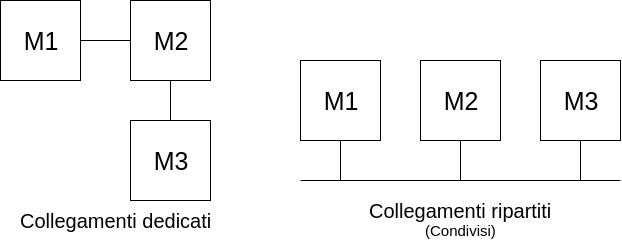
\includegraphics[scale=0.6]{strutturainterna.png}
\end{center}
\paragraph{Moduli di Elaborazione} Un modulo di elaborazione è definito come \textbf{un'entità autonoma e sequenziale}.
\subparagraph{Autonomia} L'autonomia è \textbf{data dal fatto che ogni modulo} di elaborazione \textbf{esegue un proprio controllo in maniera indipendente da altri moduli}.\\
Esso dunque \textbf{definisce le proprie strutture dati, operazioni elementari e interfacce} verso altri moduli.
\subparagraph{Sequenzialità} La sequenzialità è \textbf{data dal fatto che ogni modulo} di elaborazione \textbf{ha un singolo luogo di controllo}: \textbf{la sua attività è descritta} da un algoritmo di controllo costituito \textbf{da una lista sequenziale di comandi}.\\
La sequenzialità \textbf{non implica che un modulo non possa fare uso di forme di elaborazione concorrenti o parallele}. Alcuni o tutti i comandi di una lista sequenziale possono essere costituiti da una o più operazioni elementari \textbf{eseguite simultaneamente}.
\subsection{Parallelismo}
\paragraph{Sovrapporre} Poichè i moduli sono autonomi fra loro, sono in grado di \textbf{operare indipendentemente l'uno dall'altro}. \textbf{Le loro attività possono quindi essere sovrapposte nel tempo} eccetto quando, per ragioni legate alla sincronizzazione, alcuni di loro devono attendere il verificarsi di certi eventi dipendenti dall'elaborazione di altri.\\
In alcuni \textbf{casi limite} seppur realistici, il \textbf{funzionamento di tutti i moduli è rigidamente sequenziale}.\\\\
Tutto questo \textbf{vale per qualsiasi livello} o Macchina Virtuale, quindi sia per firmware che hardware.
\pagebreak
\subsection{Modelli di Cooperazione}
Dato un sistema di elaborazione a un certo livello, \textbf{i vari moduli} presenti \textbf{possono cooperare secondo due modalità}:
\begin{list}{}{}
	\item \textbf{Ambiente Globale}: esiste un \textbf{insieme di oggetti comuni accessibili da tutti i moduli} che devono cooperare tra loro, e \textbf{tutti i moduli possono operare su tale insieme}
	\item \textbf{Ambiente Locale}: \textbf{i moduli non condividono nulla}, quindi \textbf{non esiste alcun oggetto condivisio tra i moduli}. La \textbf{cooperazione avviene tramite scambio di messaggi}.
\end{list}
\begin{center}
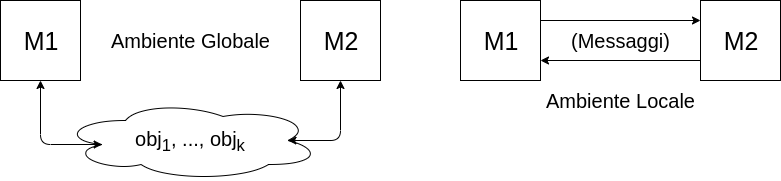
\includegraphics[scale=0.5]{modellicoop.png}
\end{center}
\pagebreak
\section{Compilazione vs Interpretazione}
\paragraph{Programmi} L'obiettivo di un calcolatore è \textbf{rendere possibile l'esecuzione di programmi} con una certa qualità di servizio. I programmi vengono \textbf{progettati mediante linguaggi di alto livello}, quindi \textbf{occorre operare una traduzione da linguaggio di alto livello a linguaggio assembler}.\\
Tale traduzione può essere effettuata tramite due ben note tecniche e loro combinazioni:
\begin{multicols}{2}
\textbf{Compilatore}: è \textbf{statico}.\\\textbf{Sostituisce l'intera sequenza del programma} sorgente con un sequenza di istruzioni assembler. Questa traduzione viene effettuata staticamente, vale a dire in fase di preparazione e \textbf{prima che il programma passi in esecuzione}.\\
Uno compilatore ha \textbf{completa visione del codice} e quindi \textbf{può ottimizzarlo}. La sua attività è analoga all'opera di un traduttore, che può leggersi il testo più volte per tradurlo alla perfezione.
\columnbreak

\textbf{Interprete}: è \textbf{dinamico}\\ Scandisce la sequenza \textbf{sostituendo ogni singolo comando} con una sequenza na di istruzioni assembler. La traduzione è effettuata dinamicamente, cioè \textbf{a tempo di esecuzione}, quindi non può ottimizzare. Il firmware riceve un'istruzione alla volta, quindi la interpreta.\\
Il suo svantaggio è che il \textbf{tempo di interpretazione viene pagato ogni volta che lancio il programma} e che \textbf{non può ottimizzare non avendo una visione globale} del programma.
\end{multicols}
Entrambe servono per tradurre il \textbf{codice sorgente} nel \textbf{programma oggetto} o \textbf{eseguibile}. L'esecuzione è quindi \textbf{più veloce in un programma compilato} rispetto ad un programma interpretato.
\begin{center}
\texttt{ADD R1, R2, R3} $\longrightarrow$ \textit{compilatore} $\longrightarrow$ \textbf{OBJ} $\longrightarrow$ Interprete Firmware (interfaccia tra MV ASM e MV FW)
\end{center}
Intuitivamente, dall'istruzione ad alto livello viene \textbf{compilato un programma oggetto OBJ} il quale è un insieme di bit che \textbf{viene interpretato dall'interprete firmware}.
\paragraph{Esempio} \textbf{Suppongo programmi}:\\
\begin{center}
	\begin{multicols}{2}
	\textbf{A}
	\begin{verbatim}
for i=0; i++; i<n
    A[i] = A[i] + B[i];
	\end{verbatim}

	\columnbreak
	\textbf{B}
	\begin{verbatim}
for i=0; i++; i<n
    B[i] = B[i] + C;
	\end{verbatim}
	\end{multicols}
\end{center}
Ricevendo i due blocchi di istruzioni, il \textbf{compilatore riconosce che sono diverse e le compila in modo diverso}. Però in entrambi i casi sono del tipo \textit{oggetto = somma due oggetti}, quindi produce una sequenza di istruzioni analoga (a meno di registri e dati, ovviamente).
Parte del secondo pezzo di codice, ad esempio, verrà tradotto in questa maniera:
\begin{multicols}{2}
\begin{list}{}{}
\item \texttt{LOAD R$_{base}$, R$_{I}$, R$_{1}$}
\item \texttt{ADD R$_{1}$, R$_{2}$, R$_{1}$}
\item \texttt{STORE R$_{base}$, R$_{I}$, R$_{1}$}
\item \texttt{INC R$_{I}$}
\item \texttt{IF$<$ R$_{I}$, R$_{N}$, LOOP}
\end{list}
\columnbreak
\begin{list}{}{}
\item \texttt{M[R[base] + R[I]] $\rightarrow$ R[1]}
\item \texttt{R[1] + R[2] $\rightarrow$ R[1]}
\item \texttt{R[1]  $\rightarrow$ M[R[base] + R[I]]}
\item \texttt{R[I] + 1 $\rightarrow$ R[I]}
\end{list}
\textbf{Microlinguaggio corrispondente}
\end{multicols}
\chapter{MV0 -- Hardware}
\section{Reti Logiche}
L'\textbf{implementazione a livello hardware di funzioni "pure"} dà luogo alle \textbf{Reti Combinatorie}.\\
L'\textbf{implementazione} a livello hardware \textbf{di funzioni "con stato"} dà luogo alle \textbf{Reti Sequenziali}.
\paragraph{Famiglia} Entrambe definiscono la famiglia delle \textbf{Reti Logiche} che permettono di \textbf{realizzare il livello hardware di un sistema di elaborazione}.
\section{Reti Combinatorie}
Una \textbf{rete combinatoria è} una rete logica \textbf{con \texttt{n} ingressi binari X$_{1}$ \ldots X$_{n}$ e \texttt{m} uscite binarie Z$_{1}$ \ldots Z$_{m}$}. Ad \textbf{ogni combinazione di valori in entrata corrisponde una ed una sola combinazione di valori in uscita}. La corrispondenza è definita secondo la funzione implementata dalla rete combinatoria.\\
Indichiamo X$_{1}$ \ldots X$_{n}$ e Z$_{1}$ \ldots Z$_{m}$ come \textbf{variabili logiche} di ingresso ed uscita. \textbf{Tutte le combinazioni possibili} delle variabili logiche \textbf{sono dette stati} di ingresso -- con 2$^n$ possibilità -- e di uscita -- 2$^m$ possibilità.\\\\
Pe rdescrivere le proprietà e la struttura interna delle reti combinatorie si usa un'\textbf{algebra isomorfa a quella logica}, chiama \textbf{Algebra Booleana}.
\subsection{Algebra Booleana}
L'algebra booleana è computata su \textbf{due valori} e \textbf{tre operatori}:
\begin{center}
\begin{multicols}{2}
\texttt{false}\\\texttt{true}\\
\columnbreak
\texttt{AND}\\\texttt{OR}\\\texttt{NOT}
\end{multicols}
\end{center}
Esistono anche altri operatori, derivati dai tre precedenti: \texttt{XOR}, \texttt{NAND}, \texttt{NOR} ecc..
\paragraph{Proprietà} Vale la proprietà distributiva anche per la somma rispetto alla moltiplicazione, oltre il viceversa, quindi: \texttt{A(B+C) = AB + AC}, ma anche \texttt{A + BC = (A + B)(A + C)}.\\
\begin{list}{-}{Inoltre si hanno le cosiddette \textbf{proprietà di DeMorgan}:}
\item \texttt{$\overline{A + B}$ = $\overline{A}$ * $\overline{B}$}
\item \texttt{$\overline{AB}$ = $\overline{A}$ + $\overline{B}$}
\end{list}
\begin{multicols}{3}
\subsubsection{AND}
Anche detta \textbf{moltiplicazione logica}.\\
\begin{tabular}{cc|c}
X & Y & Z \\
0 & 0 & 0 \\
0 & 1 & 0 \\
1 & 0 & 0 \\
1 & 1 & 1 \\
\end{tabular}
\columnbreak
\subsubsection{OR}
Anche detta \textbf{somma logica}.\\
\begin{tabular}{cc|c}
X & Y & Z \\
0 & 0 & 0 \\
0 & 1 & 1 \\
1 & 0 & 1 \\
1 & 1 & 1 \\
\end{tabular}
\columnbreak
\subsubsection{NOT}
Anche detta \textbf{negazione logica}.\\
\begin{tabular}{c|c}
Y & Z \\
0 & 1 \\
1 & 0 \\
\end{tabular}
\end{multicols}
Per costruire una \textbf{rete combinatoria} esistono varie tecniche. Quella che useremo si chiama \textbf{somma di prodotti}.
\subsection{Tecnica della Somma di Prodotti, o codifica degli 1}
\paragraph{La tecnica nel dettaglio} Partendo dalla \textbf{tabella di verità}, identifico le uscite che valgono 1. Di quelle uscite, \textbf{moltiplico (\texttt{AND})} tra loro le entrate \textbf{sulla stessa riga}, \textbf{nego le entrate che valgono 0} e \textbf{sommo (\texttt{OR}) tra loro le diverse righe}.
\paragraph{Un esempio con la somma algebrica} Partendo dalla seguente tabella di verità.\\
\begin{multicols}{2}
\begin{tabular}{cc|c|c}
X & Y & Z & R \\
0 & 0 & 0 & 0 \\
0 & 1 & 1 & 0 \\
1 & 0 & 1 & 0 \\
1 & 1 & 0 & 1\\
\end{tabular}
\columnbreak
\\Sfruttando la tecnica descritta sopra ottengo le seguenti espressioni per le due uscite:
\begin{list}{}{}
\item \texttt{Z = $\overline{X}$ * Y + X * $\overline{Y}$}
\item \texttt{R = X * Y}
\end{list}
\end{multicols}
Alternativamente, posso anche realizzare la \textbf{funzione complementare}, ovver fare il solito procedimento ma per le uscite che valgono 0 per poi negarle.\\
\begin{multicols}{2}
\begin{tabular}{cc|c|c}
X & Y & $\overline{Z}$ & R \\
0 & 0 & 1 & 0 \\
0 & 1 & 0 & 0 \\
1 & 0 & 0 & 0 \\
1 & 1 & 1 & 1\\
\end{tabular}
\columnbreak
\begin{list}{}{}
\item \texttt{Z = $\overline{\overline{X} * \overline{Y} + X * Y}$}
\item \texttt{R = X * Y}
\end{list}
\end{multicols}
\paragraph{Esempio}
\begin{center}
\begin{tabular}{cccc|c}
S1 & S2 & X & Y & S1* \\
0 & 0 & 0 & 0 & 0\\
0 & 0 & 0 & 1 & 0\\
0 & 0 & 1 & 0 & 0\\
0 & 0 & 1 & 1 & 1\\
0 & 1 & 0 & 0 & 0\\
0 & 1 & 0 & 1 & 0\\
0 & 1 & 1 & 0 & 0\\
0 & 1 & 1 & 1 & 1\\
1 & 0 & 0 & 0 & 0\\
1 & 0 & 0 & 1 & 1\\
1 & 0 & 1 & 0 & 1\\
1 & 0 & 1 & 1 & 1\\
1 & 1 & 0 & 0 & 0\\
1 & 1 & 0 & 1 & 1\\
1 & 1 & 1 & 0 & 1\\
1 & 1 & 1 & 1 & 1\\
\end{tabular}
\end{center}
S1* = $\overline{S1}$*$\overline{S2}$*X*Y + $\overline{S1}$*S2*X*Y + S1*$\overline{S2}$*$\overline{X}$*$\overline{Y}$ + S1*$\overline{S2}$*X*$\overline{Y}$ + S1*$\overline{S2}$*X*Y + S1*S2*$\overline{X}$*Y + S1*S2*X*$\overline{Y}$ + S1*S2*X*Y
\pagebreak
\subsection{Porte Logiche}
Una volta ricavata l'espressione logica dalla tabella di verità, è \textbf{immediato realizzare lo schema logico utilizzando le componenti hardware elementari}, dette anche \textbf{porte logiche}:
\begin{center}
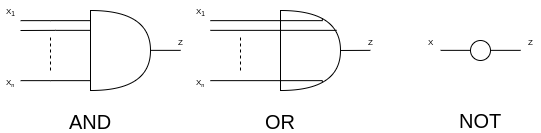
\includegraphics[scale=0.9]{portelogiche.png}
\end{center}
Ogni porta logica AND e OR \textbf{comporta un ritardo nel calcolo di 1 T$_p$}. Inoltre, ogni AND e OR può avere \textbf{massimo 8 ingressi}, quindi se ho più di 8 segnali in ingresso devo avere \textit{almeno} due livelli: un livello con tante porte logiche quando n/8 con n numero di segnali in ingresso, e \textit{almeno} un livello in cui "unire" i segnali in uscita in una porta logica analoga.
\subsection{Componenti Standard}
Di seguito sono le specifiche di alcune \textbf{reti combinatorie} che verranno supposte come \textbf{standard}, ovvero come componenti utilizzabili come blocchi elementari nella progettazione di strutture più complesse.
\subsubsection{Commutatore}
	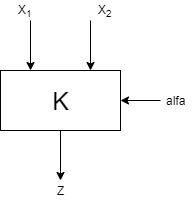
\includegraphics[scale=0.7]{commutatore.png}
\subsubsection{Selezionatore}
	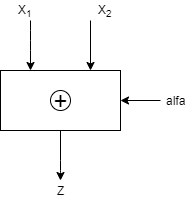
\includegraphics[scale=0.7]{confrontatore.png}
\subsubsection{Confrontatore}
	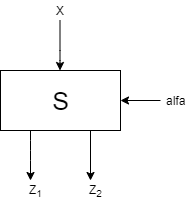
\includegraphics[scale=0.7]{selezionatore.png}
\subsubsection{ALU}
	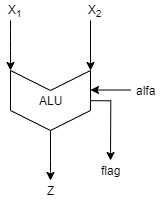
\includegraphics[scale=0.7]{ALU.png}
\subsection{Ritardo di Stabilizzazione}
\paragraph{Prestazioni} Per valutare le prestazioni di un sistema, occorre saper \textbf{valutare le prestazioni delle reti combinatorie}. Ogni rete reale è \textbf{caratterizzata da un ritardo T$_r$}, necessario affinché \textbf{a seguito di una variazione dello stato d'ingresso si produca la corrispondente variazione dello stato in uscita}.\\
\textbf{Solo dopo} questo tempo si dice che \textbf{la rete è stabilizzata}.
\paragraph{T$_p$} Per una porta logica indichiamo con T$_p$ \textbf{il ritardo di stabilizzazione} -- ad oggi è di circa 10$^{-2}$ millisecondi.\\
Supponiamo che le \textbf{porte NOT} abbiano un \textbf{ritardo nullo}, pari a 0 T$_p$, mentre per le \textbf{porte AND/OR} il valore T$_p$ dipende dal numero di ingressi n della porta. Per n $\leq$ 8 supponiamo che le porte AND/OR abbiano un \textbf{ritardo di stabilizzazione di 1 T$_p$}.\\
Il costo in T$_p$ sarà quindi pari ai livelli di AND/OR presenti. Ad esempio, se ho una tabella di verità con n termini ed m variabili, avrò log$_8$n livelli di OR e log$_8$m livelli di AND. Il costo in T$_p$ sarà quindi = (log$_8$n + log$_8$m) T$_p$
\subsection{Registri e memorie}
\pagebreak
\section{Reti Sequenziali}
Una \textbf{rete sequenziale} è un oggetto con \textbf{un ingresso ed una uscita}, capace di \textbf{mantenere uno stato interno} -- ecco perché si parla di funzioni con stato. A livello hardware, possiamo identificare una rete sequenziale con un \textbf{automa a stati finiti}.
\paragraph{ASF} Un \textbf{automa a stati finiti} è caratterizzato da:
\begin{list}{}{}
	\item n variabili di ingresso $\Rightarrow$ h = 2$^n$ \textbf{stati di ingresso} X$_1$\ldots X$_h$
	\item m variabili di uscita $\Rightarrow$ k = 2$^m$ \textbf{stati di uscita} Z$_1$\ldots Z$_k$
	\item r variabili logiche dello stato interno $\Rightarrow$ p = 2$^r$ \textbf{stati interni} S$_1$\ldots S$_p$
	\item una \textbf{funzione di transizione} dello stato interno $\sigma$: X x S $\rightarrow$ S che \textbf{definisce il passaggio tra gli stati}
	\item una \textbf{funzione delle uscite} $\omega$: X x S $\rightarrow$ Z che \textbf{calcola le uscite}
\end{list}
Una \textbf{rete sequenziale} è quindi \textbf{composta da due reti combinatorie $\sigma$ e $\omega$}, che rispettivamente calcolano la variazione dello stato e l'uscita, \textbf{e da un registro R} che contiene lo stato interno.
\subsection{Modello di Mealy}
\begin{multicols}{2}
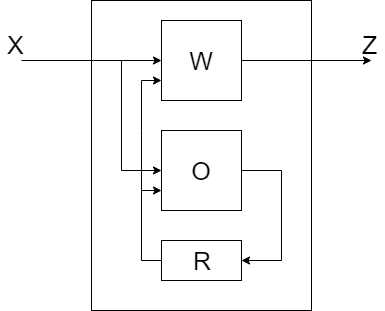
\includegraphics[scale=0.5]{mealy.png}
\columnbreak

Considerando il comportamento al tempo t, lo \textbf{stato interno successivo S(t+1)} dipende sia dallo stato di ingresso al tempo t, cioè X(t), sia dallo stato interno attuale S(t).\\
\texttt{S(t+1) = $\sigma$(X(t), S(t))}\\\\

Lo \textbf{stato di uscita al tempo t, Z(t)}, dipende sia dallo stato di ingresso X(t) sia dallo stato interno attuale S(t).\\
\texttt{Z(t) = $\omega$(X(t), S(t))}\\\\
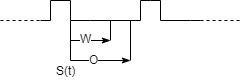
\includegraphics[scale=0.8]{clockmemo.png}
\end{multicols}
\subsection{Modello di Moore}
\begin{multicols}{2}
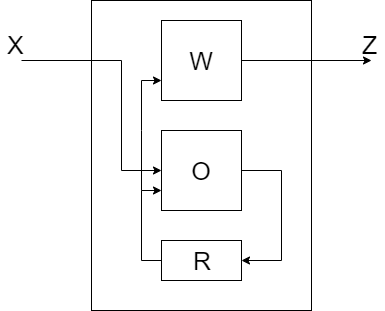
\includegraphics[scale=0.5]{moore.png}
\columnbreak

In maniera analoga al modello di Mealy, lo \textbf{stato interno successivo S(t+1)} dipende sia dallo stato di ingresso al tempo t, cioè X(t), sia dallo stato interno attuale S(t).\\
\texttt{S(t+1) = $\sigma$(X(t), S(t))}\\\\

Lo \textbf{stato di uscita al tempo t, Z(t)}, dipende solo dallo stato interno attuale S(t).\\
\texttt{Z(t) = $\omega$(S(t))}\\\\
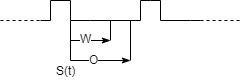
\includegraphics[scale=0.8]{clockmemo.png}
\end{multicols}
\pagebreak
\subsection{Reti Sequenziali di tipo Sincrono}
Vediamo adesso come si comportano nel tempo le reti sequenziali e spieghiamo perché adotteremo quelle di tipo sincrono. Come riferimento usiamo una rete di Mealy.
\paragraph{Spezzare} Abbiamo detto che lo stato al tempo successivo S(t + 1) dipende sia dall'ingresso X sia dallo stato interno attuale S(t), cioè \texttt{S(t+1) = $\sigma$(X(t), S(t))}.\\
Il registro R funge come un "cancello temporizzato" che \textbf{spezza la sequenza temporale degli eventi}.
\begin{multicols}{2}
Se il registro R non fosse presente, si verificherebbe la situazione in figura. In questo esempio, la porta logica o il componente $\sigma$ \textbf{potrebbero non stabilizzarsi mai}.\\
Se per esempio mettiamo una porta AND con due variabili in ingresso che nega il proprio risultato, tale rete tenderà a non stabilizzarsi mai ma a produrre una sequenza infinita di 0 e 1 in uscita.\\
Quindi devo avere necessariamente \textbf{un meccanismo che mi possa aiutare a determinare il valore dell'uscita} al tempo t, t + 1\ldots\\\\
Questo strumento è il resgistro impulsato, dove \textbf{la scrittura è scandita dal ciclo di clock}.
\columnbreak

\begin{center}
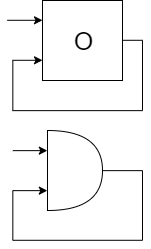
\includegraphics[scale=0.6]{esempiosincrono.png}
\end{center}
\end{multicols}
\paragraph{Modo Sincrono} Questo modo di lavorare delle reti sequenziali con un registro impulsato che funge da cancello temporizzato grazie al ciclo di clock si chiama \textbf{Modo Sincrono}.
\paragraph{Quando variare} Cerchiamo ora di capire quando devono variare gli ingressi e \textbf{per quanto tempo devono avere tale valore}.\\
Supponiamo di avere gli ingressi X$_0$ = 0 al tempo t, X$_1$ = 1 al tempo t + 1 e X$_2$ = 0 al tempo t + 2, e supponiamo che t$_\omega$ = t$_\sigma$ = 2t.
\begin{multicols}{2}
Se l'ingresso X variasse in un punto non precisato del ciclo di clock è probabile che $\omega$ e $\sigma$ non abbiano il \textbf{tempo necessario per produrre un risultato} e quindi avrei un \textbf{comportamento indefinito}.\\\\\\\\\\
In questo caso, cambiando il valore X all'inizio del ciclo di clock do il tempo necessario a $\sigma$ e $\omega$ di produrre un risultato stabile, ma al prossimo impulso del ciclo di clock (t + 2) leggerò di nuovo X = 1, che non è l'input corretto al tempo t + 2.\\\\\\\\\\\\
Questa è la soluzione giusta per il nostro esempio, che rispetta tutte le condizioni da noi elencate.
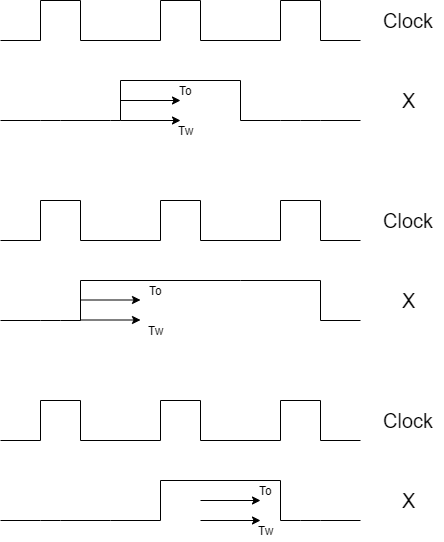
\includegraphics[scale=0.5]{sincronoesempi.png}
\end{multicols}
Per far funzionare le nostre reti, il ciclo di clock deve essere tale che T = MAX(t$_\sigma$, t$_\omega$) + $\delta$. Le reti funzionano anche con T $>$ MAX(t$_\sigma$, t$_\omega$) + $\delta$, ma avrei del \textbf{tempo perso} poiché la rete non opera, \textbf{aspetta solo che il clock sia alto per andare a scrivere nel registro}.
\pagebreak
\subsection{Reti Sequenziali a Componenti Standard}
Per poter sintetizzare una rete devo prima \textbf{decidere} se \textbf{implementare un modello di Mealy o di Moore}, \textbf{derivare le tabelle di verità} di $\omega$ e $\sigma$ e dire \textbf{quanti bit} ha il registro R.\\
Fatto questo, \textbf{ricavare le reti combinatorie} e \textbf{capire quanto valga il ciclo di clock} T (con T = MAX(t$_\sigma$, t$_\omega$) + $\delta$) che fa funzionare l'intera rete sequenziale.
\paragraph{Sintesi Classica} ASF $\longrightarrow$ Mealy o Moore $\rightarrow$ Tabelle verità, bit di R $\Rightarrow$ Reti combinatorie $\Rightarrow$ Ciclo di clock
\paragraph{Componenti Standard} In realtà per sintetizzare le reti sequenziali non usiamo questo procedimento di sintesi, ma bensì \textbf{usiamo i componenti standard}. Per esempio, prendiamo una rete che vuole calcolare il numero di persone presenti dentro una stanza con capienza massima 100 persone.
\paragraph{Con la sintesi classica} R ha bisogno di 7 bit per contare da 0 a 100.\\
Se andiamo, per esempio, a fare la tabella di verità per $\omega$, abbiamo ben 8 colonne negli ingressi, quindi 2$^8$ possibili combinazioni (righe).\\
Potrei avere 2$^8$/2 = 2$^7$ "uni" per colonna, di conseguenza un \textbf{numero considerevole di porte logiche}.\\
Diventa quindi praticamente impossibile sintetizzare questo esempio con il metodo classico. Procediamo con l'alternativa: l'utilizzo delle componenti standard.
\paragraph{Con le componenti standard} Procediamo col nostro esempio:\\
\begin{multicols}{2}
\begin{center}
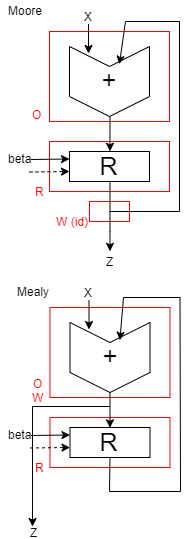
\includegraphics[scale=0.8]{esempiocompstd.png}
\end{center}
\columnbreak

In questo caso abbiamo usato il modello di Moore. Il \textbf{risultato è disponibile al prossimo impulso del ciclo di clock}.\\\\\\\\\\\\\\\\\\\\\\\\\\\\\\\\\\\\

Qua invece è stato usato il modello di Mealy. In questo caso si vede bene come \textbf{la rete di Mealy sia più veloce}, poiché \textbf{il risultato è subito disponibile} prima del prossimo impulso del ciclo di clock: infatti Z non viene scritto in R prima di essere pubblicato.
\end{multicols}
\pagebreak
Di seguito un esempio di rete sequenziale a componenti standard più complesso.
\begin{center}
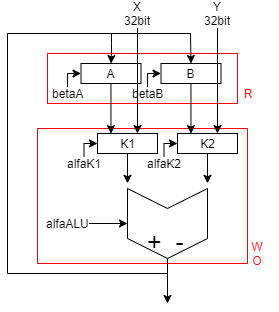
\includegraphics[scale=0.8]{compstdesempiobig.png}
\end{center}
\paragraph{Con sintesi classica} Avrei:
\begin{list}{}{}
	\item R = \{A, B\}, due registri da 32 bit $\Rightarrow$ 64 bit
	\item Ingressi: X + Y + $\alpha_{K1}$ + $\alpha_{K2}$ + $\alpha_{ALU}$ + $\beta_A$ + $\beta_B$ = 32 + 32 + 3 + 2 = 69
	\item Uscite: Z $\Rightarrow$ 32 bit
\end{list}
La tabella di verità di $\omega$, per esempio, avrebbe 69 colonne di ingressi, quindi 2$^{69}$ righe, \textbf{senza considerare gli ingressi di A e B}.\\
Il risultato è che è molto scomodo lavorare con una tabella di circa 5.9 * 10$^{20}$ righe.
\pagebreak
\chapter{MV1 -- Firmware}
\section{Unità Firmware}
Un sistema di elaborazione, a livello Firmware, è costituito da un certo numero di \textbf{Unità Firmware} che interagiscono fra loro mediante un sistema di interconnessione. Le UF sono capaci si svolgere un certo numero di operazioni esterne.
\paragraph{Unità Firmware} Una \textbf{unità firmware} è un \textbf{modulo di elaborazione autonomo} -- cioè capace di controllare la propria operazione in modo del tutto indipendente -- \textbf{e sequenziale} -- cioè dal funzionamento descritto da un programma sequenziale -- \textbf{capace di eseguire delle operazioni esterne} -- istruzioni \textbf{assembler}.
\paragraph{Struttura di interconnessione} Tipicamente la struttura di interconnessione tra unità firmware è \textbf{punto-a-punto} quindi a \textbf{collegamenti dedicati}.
\subsection{PC e PO}
Per capire bene cosa sono e a cosa servono le parti controllo (PC) e operativa (PO), vediamo un semplice esempio di come arriviamo a strutturare un'unità firmware.
\begin{center}
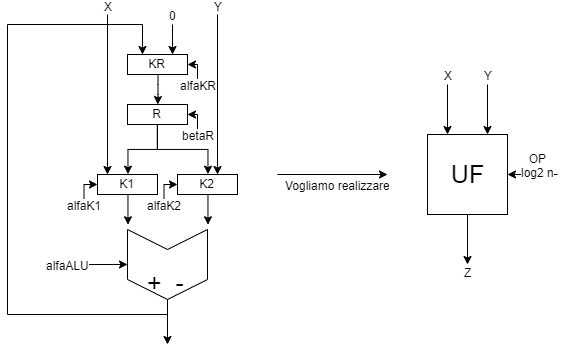
\includegraphics[scale=0.6]{ufesempio.png}
\end{center}
Il nostro obiettivo è quello di realizzare una unità capace di produrre un risultato Z a partire dalle variabili in input, \textbf{fornendogli solo le istruzioni per l'operazione da implementare} e \textbf{capace di gestire tutte le variabili di controllo} ($\alpha$, $\beta$) \textbf{in maniera autonoma}.\\
L'unità firmware è quindi l'unione di due oggetti:
\begin{list}{}{}
\item \textbf{Parte Controllo} che "comanda" l'operazione da eseguire
\item \textbf{Parte Operativa} che "esegue" l'operazione
\end{list}
\pagebreak
\subsubsection{Ciclo di Clock}
\begin{center}
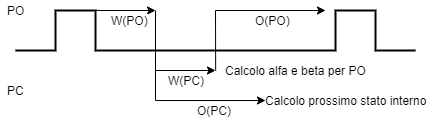
\includegraphics[scale=1]{ufclock.png}
\end{center}
PO e PC sono\textbf{reti sequenziali impulsate} dallo stesso segnale di clock, quindi aventi lo stesso ciclo di clock. Il \textbf{ciclo di clock dell'unità firmware} viene determinato in modo da \textbf{permettere la stabilizzazione di entrambe le reti per l'esecuzione di una qualsiasi microisitruzione}.\\
Questo modello di programmazione è \textbf{sincrono}.\\\\
\textbf{Schematizzazione} del diagramma del ciclo di clock sopra:
\begin{list}{}{}
	\item $\omega_{PO}$: prepara i valori che servono alla PC per decidere cosa fare
	\item $\omega_{PC}$: prepara \{$\alpha$, $\beta$\} che implementano l'operazione richiesta
	\item $\sigma_{PC}$: decido il prossimo stato interno della PC $\rightarrow$ scrivo il registro R della PC
	\item $\sigma_{PO}$: eseguo l'operazione pianificata $\rightarrow$ scrivo i nuovi valori nei registri che compongono lo stato interno della PO
\end{list}
\subsubsection{Parte Operativa, Moore}
\textbf{Rete Sequenziale} progettata con \textbf{componenti standard} che provvede all'esecuzione di \textbf{istruzioni} tramite commutatori, selettori, ALU e registri.
\subsubsection{Parte Controllo, Mealy}
\textbf{Rete Sequenziale} progettata tramite \textbf{sintesi classica} che provvede a determinare le \textbf{variabili di controllo} $\alpha$ e $\beta$ per la parte operativa.
\subsubsection{Mealy o Moore?}
Essendo entrambe due reti sequenziali bisogna decidere quale modello usare. Analizziamo le varie combinazioni di modelli.
\paragraph{Mealy--Mealy} Se uso un modello Mealy--Mealy le uscite di $\omega_{PO}$ vanno direttamente nella $\omega_{PC}$ e le uscite di $\omega_{PC}$ ritornano in $\omega_{PO}$. Non ho un registro che ferma il ciclo continuo tra $\omega_{PC}$  e $\omega_{PO}$, quindi non riuscirò mai a stabilizzare i segnali che si scambiano PO e PC.\\
Viene naturale pensare di farle entrambe Mealy--Mealy poiché, come visto in precedenza, il modello di Mealy è più veloce di quello di Moore.
\paragraph{Almeno una Moore} Concludiamo che almeno una tra PC e PO deve essere di Moore per poter stabilizzare l'intera UF, ma quale?\\
La risposta corretta è usare il \textbf{modello di Mealy per la Parte Controllo} e il \textbf{modello di Moore per la Parte Operativa} in modo da avere dei \textbf{comandi veloci} ed una \textbf{esecuzione più lenta} rispetto alla PC.
\paragraph{Il contrario?} Non scegliamo un modello Moore per PC e Mealy per PO perché è \textbf{illogico avere un esecutore veloce che deve aspettare un controllore lento}: inutile avere una macchina molto veloce se inserisco i comandi molto lentamente.\\
Anche un modello Moore--Moore non è comodo da usare, seppure funzionante correttamente, perché avrei entrambe le parti lente.
\pagebreak
\begin{multicols}{2}
	\begin{center}
		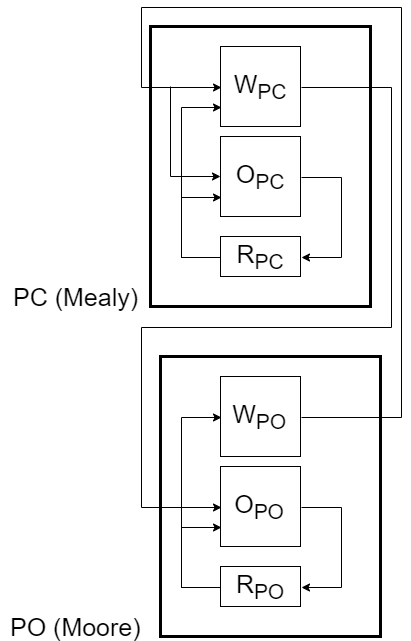
\includegraphics[scale=0.5]{pcposchema.png}
	\end{center}
	\columnbreak
	\begin{center}
		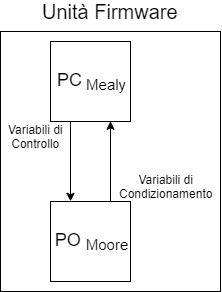
\includegraphics[scale=1]{ufschema.png}
	\end{center}
\end{multicols}
\paragraph{Condizione di Correttezza} $\Rightarrow$ PO di Moore\\
Le uscite della Parte Operativa, cioè le variabili di condizionamento, dipendono esclusivamente dallo stato interno di PO, cioè \textbf{tutte le variabili di condizionamento devono essere prodotte senza usare alcun $\alpha$}
\subsection{Procedimento Formale}
Schematizzazione dei passaggi del procedimento formale per la costruzione e l'analisi di una rete sequenziale.
\begin{enumerate}
	\item Descrizione a parole delle operazioni esterne
	\item Programma scritto in $\mu$-linguaggio
	\item Componenti
	\begin{list}{}{}
		\item R$_{PO}$: capire quali sono i registri di stato della PO
		\item $\omega_{PO}$, $\sigma_{PO}$: capire le funzioni che mi servono nella PO
		\item R$_{PC}$: capire cosa è lo stato della PC
		\item $\omega_{PC}$, $\sigma_{PC}$: capire cosa calcolare nella PC
		\item $\longrightarrow$ T = t($\omega_{PO}$) + MAX\{t($\omega_{PC}$) + t($\sigma_{PO}$), t($\omega_{PC}$)\} + $\delta$
	\end{list}
\end{enumerate}
\pagebreak
\chapter{$\mu$-linguaggio}
Si formalizza un linguaggio chiamato \textbf{$\mu$-linguaggio} che permetta di \textbf{derivare formalmente com'è fatta la PC e la PO di una certa UF}.
\section{Istruzioni}
Nel $\mu$-linguaggio sono presenti solamente \textbf{due tipi di istruzione}:
\begin{list}{}{}
	\item \texttt{n. $\mu$op$_1$, \ldots, $\mu$op$_k$, m}\\
	Le \texttt{op} sono \textbf{operazioni di trasferimento tra registri}. Le varie \texttt{op} \textbf{separate da una virgola sono eseguite contemporaneamente} -- cioè nello stesso ciclo di clock.\\
	\texttt{m} finale indica \textbf{a quale istruzione andare dopo aver eseguito questa istruzione}, la \texttt{n}.
	\item \texttt{n. (condizione = T) $\mu$op$_1$, \ldots, $\mu$op$_k$, m'\\
	(condizione = F) $\mu$op$_1$, \ldots, $\mu$op$_h$, m''}\\
	Le \textbf{condizioni} sono \textbf{date in termini di variabili di condizionamento}. Possono essere messe in sequenza, venendo \textbf{valutate in sequenza}.\\
	Posso considerare solo \textbf{variabili booleane} o \textbf{espressioni di cui mi interessa solo il risultato} senza memorizzarlo.
\end{list}
\paragraph{Esempio} Vediamo un esempio di come scrivere un programma in $\mu$-linguaggio. Prendiamo come esempio la divisione fra interi.\\
\begin{multicols}{2}
\begin{center}
\textbf{Linguaggio pseudo-C}
\begin{verbatim}
Q = 0
while (A >= B) {
    Q = Q + 1
    A = A - B
}
R = A
\end{verbatim}
\end{center}
\columnbreak
\begin{center}
\textbf{$\mu$-linguaggio}
\begin{lstlisting}
0.  0 -> Q, 1
1.  (segno(A - B) = 0) nop, 2
    (= 1)              nop, 4
2.  Q + 1 -> Q, 3
3.  A - B -> A, 1
4.  A -> R, 0
\end{lstlisting}
\end{center}
\end{multicols}
Ogni $\mu$-istruzione è \textbf{eseguita esattamente in un ciclo di clock}. Nell'esempio, per eseguire il programma avrò bisogno di almeno 5 cicli di clock, a meno di iterazioni interne.
\pagebreak
\section{Ottimizzazione del codice}
Dopo aver scritto il $\mu$-codice possiamo provare ad \textbf{ottimizzarlo}, cioè \textbf{ridurre il numero di cicli di clock necessari ad eseguirlo}.\\
Un'ottimizzazione possibile dell'esempio precedente è la seguente.
\begin{multicols}{2}
\begin{center}
Prima
\begin{lstlisting}
0.  0 -> Q, 1
1.  (segno(A - B) = 0) nop, 2
    (= 1)              nop, 4
2.  Q + 1 -> Q, 3
3.  A - B -> A, 1
4.  A -> R, 0
\end{lstlisting}
\end{center}
\columnbreak
\begin{center}
Dopo
\begin{lstlisting}
0.  0 -> Q, A - B -> T, A - B -> A, 1
1.  (T0 = 0) Q + 1 -> Q, A - B -> A, A - B -> T, 1
    (= 1)    A -> R, 0
\end{lstlisting}
\end{center}
\end{multicols}
Considero un registro T dove memorizzo il risultato di A - B. Di quel registro T, considero T$_0$ -- cioè il bit più significativo -- per il segno.\\
Inoltre elimino le \texttt{nop}, che sono \textit{tempo sprecato}.
\subsection{Condizioni di Bernstein}
Per eseguire le ottimizzazioni sul $\mu$-codice, dobbiamo \textbf{seguire le Condizioni di Bernstein}. Tali condizioni forniscono delle regole per verificare se due o più $\mu$-operazioni possono essere eseguite nella medesima $\mu$-istruzione.
\paragraph{Le Condizioni} Per capire se\\
\texttt{i. $\mu$op$_A$, i+1\\
i+1. $\mu$op$_B$, k}\\
è equivalente a\\
\texttt{i. $\mu$op$_A$, $\mu$op$_B$, k}\\
Bisogna \textbf{valutare il dominio R(op)} -- registri \textbf{letti} da op -- e \textbf{il codominio W(op)} -- registri \textbf{scritti} da op -- delle $\mu$-operazioni.\\
Nell'esempio precedente:
\begin{list}{}{}
	\item R(A - B $\rightarrow$ T) = \{A, B\}
	\item W(A - B $\rightarrow$ T) = \{T\}
	\item R(Q + 1 $\rightarrow$ Q) = \{Q\}
	\item W(Q + 1 $\rightarrow$ Q) = \{Q\}
\end{list}
Le \textbf{condizioni da verificare} sono:
\begin{list}{}{}
	\item W($\mu$op$_A$) $\cap$ R($\mu$op$_B$) = $\emptyset$\\
	\textbf{Dipendenza}: non posso mettere insieme $\mu$-operazioni tali che la prima scrive in un registro letto dalla seconda.
	\item W($\mu$op$_A$) $\cap$ W($\mu$op$_B$) = $\emptyset$\\
	\textbf{Dipendenza di output}: non posso scrivere nello stesso registro con due $\mu$-operazioni diverse nella stessa $\mu$-istruzione.
\end{list}
\subsection{Variabili di Condizionamento}
Le \textbf{variabili di condizionamento} possono essere così categorizzate:
\begin{list}{}{}
	\item \textbf{Semplici}: indicano le uscite di registri \textbf{senza trasformazioni}\\
	$\longrightarrow$ t$_{\omega PO}$ = 0
	\item \textbf{Complesse}: indicano \textbf{trasformazioni delle uscite di registri} fatte tramite reti combinatorie prive di ingressi di controllo.\\
	Esempio: \texttt{segno(A - B)}, \texttt{OR(A)}\\
	$\longrightarrow$ t$_{\omega PO}$ = k t$_p$
\end{list}
\pagebreak
\subsection{Tempo medio di elaborazione}
Il \textbf{tempo medio di elaborazione} di una UF viene valutato come: \texttt{$T = \sum_{i = 0}^{n - 1}(p_i * k_i) $}\\
Dove:
\begin{list}{}{}
	\item $k_i$ è il numero medio di cicli di clock necessari per eseguire una generica operazione i
	\item $p_i$ è la probabilità di eseguire tale operazione
\end{list}
Quando non sono note le $p_i$, si assume che tutte le sottosequenze siano equiprobabili. Calcoliamo quindi T come media aritmetica dei $k_i$, oppure si cerca di stimare se possibile una distribuzione probabilistica attendibile.
\subsection{Riflessioni finali sull'ottimizzazione}
Bisogna prestare particolare attenzione quando si ottimizza il $\mu$-codice. Ridurre il numero di $\mu$-istruzioni ($k_i$) non è sempre qualcosa di buono.\\
Talvolta, \textbf{unire due o più $\mu$-istruzioni obbliga ad aumentare il ciclo di clock T} per consentire al $\mu$-programma di eseguirle tutte. Questa modifica, che si applica a \textbf{tutte} le $\mu$-istruzioni, potrebbe aumentare il tempo medio di elaborazione T, rendendo il programma complessivamente più lento.\\\\
Concludendo, le ottimizzazioni che si possono fare sono:
\begin{list}{}{}
	\item Eliminare le \texttt{nop}, tranne quelle di attesa per operazioni esterne
	\item Raggruppare le $\mu$-operazioni, attraverso le condizioni di Bernstein
	\item Raggruppare le condizioni logiche
\end{list}
\section{Controllo Residuo}
Per diminuire ulteriormente la complessità della PC possiamo \textbf{delegare alla PO alcune delle decisioni che dovrebbe prendere la PC}.\\
Vediamo alcuni esempi:
\begin{list}{}{}
	\item Leggere il k-esimo bit di un registro R di n bit
	\begin{multicols}{2}
	\begin{center}
	\textbf{Soluzione classica}\\
	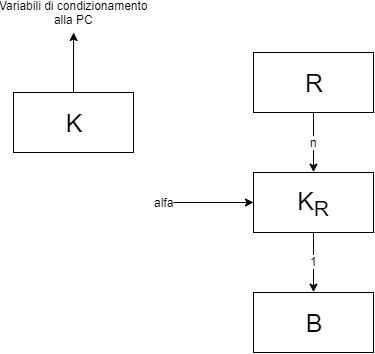
\includegraphics[scale=0.5]{contrres_es1.png}
	\end{center}
	\columnbreak
	\begin{center}
	\textbf{Controllo residuo}\\
	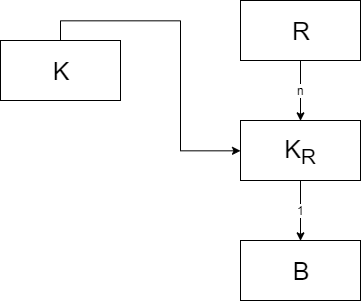
\includegraphics[scale=0.5]{contrres_es1b.png}
	\end{center}
	Risparmio complessità della PC e riduco il traffico di dati da PO a PC
	\end{multicols}
	\pagebreak
	\item Supponiamo una $\mu$-istruzione da eseguire a seconda di una certa condizione, ad esempio: \texttt{(A$_0$ = 0) B + C $\rightarrow$ D}
	\begin{multicols}{2}
	\begin{center}
	\textbf{Soluzione classica}\\
	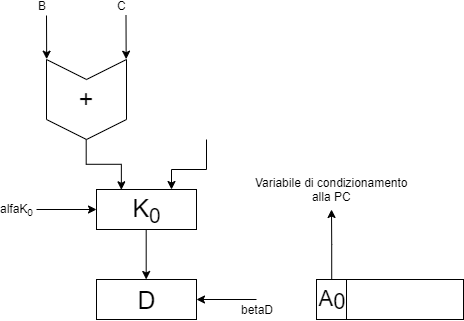
\includegraphics[scale=0.5]{contrres_es2.png}
	\end{center}
	\columnbreak
	\begin{center}
	\textbf{Controllo residuo}\\
	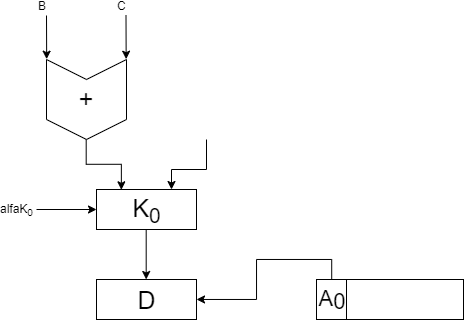
\includegraphics[scale=0.5]{contrres_es2b.png}
	\end{center}
	\end{multicols}
	\item \texttt{(segno(A - B) = 0) B - A $\rightarrow$ C\\(= 1) B + A $\rightarrow$ C}
	\begin{multicols}{2}
	\begin{center}
	\textbf{Soluzione classica}\\
	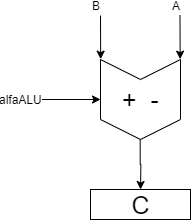
\includegraphics[scale=0.5]{contrres_es3.png}
	\end{center}
	\columnbreak
	\begin{center}
	\textbf{Controllo residuo}\\
	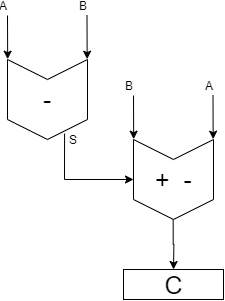
\includegraphics[scale=0.5]{contrres_es3b.png}
	\end{center}
	\end{multicols}
\end{list}
\section{Comunicazioni}
Con \textbf{comunicazioni} si intendono le \textbf{comunicazioni fra unità firmware e mondo esterno} e viceversa.\\
Nell'esempio preso in esame, della divisione fra A e B interi con Q ed R risultati, \textbf{A e B provengono dal mondo esterno e Q ed R sono comunicati verso di esso}.
\begin{center}
A,B $\longrightarrow$ UF $\longrightarrow$ Q,R
\end{center}
\paragraph{Categorie} Le comunicazioni sono \textbf{classificate in due categorie}:
\begin{list}{}{}
	\item \textbf{Simmetriche/Asimmetriche}\\
	Simmetriche: un solo mittente, un solo destinatario (\textbf{uno-a-uno})\\
	Asimmetriche: asimmetria in ingresso (\textbf{più mittenti}) o in uscita (\textbf{più destinatari})
	\item \textbf{Sincrone/Asincrone}\\
	Sincrone: la comunicazione avviene "\textbf{istantaneamente}"\\
	Asincrone: il destinatario legge il messaggio \textbf{dopo del tempo} (es. e-mail)
\end{list}
\pagebreak
\subsection{Protocollo a Livelli}
\textbf{Simmetrico e asincrono}, il protocollo a livelli \textbf{funziona aggiungendo ai registri} XOUT di UF$_1$ e XIN di UF$_2$ \textbf{altri due registri da 1 bit ciascuno}, che \textbf{indicano quando avviene la comunicazione}: \textbf{ACK e RDY}
\begin{center}
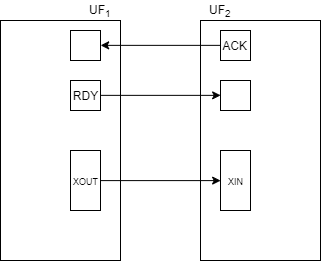
\includegraphics[scale=0.7]{ufprotliv.png}
\end{center}
Di seguito i passi del funzionamento del protocollo:
\begin{list}{}{}
	\item 1. UF$_1$ scrive XOUT e il primo registro da 1 bit
	\begin{multicols}{2}
		\begin{center}
		Situazione iniziale\\
		\begin{tabular}{ c c c }
			 0 &   & 0 \\ 
			 1 & $\longrightarrow$ & 0
		\end{tabular}
		\end{center}
		\columnbreak
		\begin{center}
		Situazione finale\\
		\begin{tabular}{ c c c }
			 0 &   & 0 \\ 
			 1 & $\longrightarrow$ & 1
		\end{tabular}
		\end{center}
		1 in RDY di UF$_2$ significa che ci sono dati significativi in XIN
	\end{multicols}
	\item 2. UF$_2$ utilizza XIN e comunica che ha finito scrivendo nel proprio registro di OUT da 1 bit
	\begin{multicols}{2}
		\begin{center}
		Situazione iniziale\\
		\begin{tabular}{ c c c }
			 0 & $\longleftarrow$ & 1 \\ 
			 1 & $\longrightarrow$ & 0
		\end{tabular}
		\end{center}
		\columnbreak
		\begin{center}
		Situazione finale\\
		\begin{tabular}{ c c c }
			 1 & $\longleftarrow$ & 1 \\ 
			 1 & $\longrightarrow$ & 1
		\end{tabular}
		\end{center}
	\end{multicols}
	\item 3/4. Ritorno alla situazione iniziale con tutti i registri da un bit a 0
	\begin{multicols}{4}
		\begin{center}
		\begin{tabular}{ c c c }
			 1 & $\longleftarrow$ & 1 \\ 
			 0 & $\longrightarrow$ & 1
		\end{tabular}
		\end{center}
		\columnbreak
		\begin{center}
		\begin{tabular}{ c c c }
			 1 & $\longleftarrow$ & 1 \\ 
			 0 & $\longrightarrow$ & 0
		\end{tabular}
		\end{center}
		\columnbreak
		\begin{center}
		\begin{tabular}{ c c c }
			 1 & $\longleftarrow$ & 0 \\ 
			 0 & $\longrightarrow$ & 0
		\end{tabular}
		\end{center}
		\columnbreak
		\begin{center}
		\begin{tabular}{ c c c }
			 0 & $\longleftarrow$ & 0 \\ 
			 0 & $\longrightarrow$ & 0
		\end{tabular}\\
		Si può riniziare
		\end{center}
	\end{multicols}
\end{list}
Vediamo i cicli di clock necessari per usare questo protocollo:
\begin{enumerate}
	\item UF$_1$ scrive 1
	\item UF$_2$ vede 1 $\rightarrow$ \ldots UF$_2$ agisce\ldots $\rightarrow$ UF$_2$ scrive 1
	\item UF$_1$ vede 1 di ritorno $\rightarrow$ UF$_1$ scrive 0
	\item UF$_2$ vede 0 $\rightarrow$ UF$_2$ scrive 0\\
	$\Rightarrow$ Condizioni iniziali: \textbf{4 cicli di clock}
\end{enumerate}
Se le due UF hanno clock sfasati uso lo stesso ragionamento, probabilmente finendo per dover usare più cicli di clock.
\paragraph{Nel programma} Come rendere questo meccanismo nel $\mu$-codice? Proviamo a scriverlo per UF$_2$:
\begin{lstlisting}
0.  (RDY = 0) nop, 0
    (= 1)     A -> TEMPA, B -> TEMPB, 1 -> ACK, 1
1.  (RDY = 1) nop, 0
    (= 0)     0 -> ACK, <proseguo con altro>
\end{lstlisting}
\pagebreak
Questo protocollo è particolarmente semplice e necessita \textbf{pochissimo hardware}, ma \textbf{richiede troppi cicli di clock per comunicare}. Vediamo un'alternativa migliore.
\subsection{Protocollo a Transizione di Livello}
\textbf{Simmetrico e asincrono}, simile al protocollo a livelli ma \textbf{usa degli indicatori di transizione di livello}.
\begin{center}
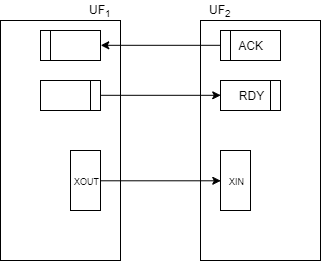
\includegraphics[scale=0.7]{uftransliv.png}
\end{center}
\subparagraph{ACK} \textbf{Contatore in modulo 2}, quindi cambia stato (0 $\leftrightarrow$ 1) ogni volta che ci scrivo.
\begin{multicols}{2}
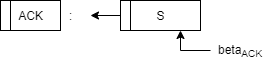
\includegraphics[scale=1]{ack.png}
\begin{center}
\begin{tabular}{ c c | c }
			 S & $\beta$ & S' \\
			 \hline
			 0 & 0 & 0 \\
			 0 & 1 & 1 \\
			 1 & 0 & 1 \\
			 1 & 1 & 0
\end{tabular}
\end{center}
\end{multicols}
\subparagraph{RDY} Risultato di un confrontatore fra un contatore modulo 2 e un registro in ingresso.
\begin{multicols}{2}
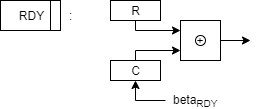
\includegraphics[scale=1]{rdy.png}
\end{multicols}
\paragraph{Funzionamento} Dal punto di vista di UF$_2$.\\
Quando arriva un segnale da UF$_1$, la rete RDY diventa 1, quindi si può lavorare con i dati ricevuti.\\
Per comunicare a UF$_1$ che l'operazione è conclusa, mando un $\beta_{ACK}$ = 1 al mio ACK, che diventerà 1 anche in uscita.\\\\
Questo procedimento è il medesimo del protocollo a livelli visto in precedenza. Quello che cambia è come mi riporto nelle condizioni iniziali.\\
Dopo aver lavorato con XIN, chiamo \texttt{reset RDY} che \textbf{riporta la rete RDY a 0}, quindi pronta ad accogliere un nuovo messaggio.\\
In poche parole, torno alle impostazioni iniziali nello stesso momento in cui ricevo il messaggio.
\pagebreak
\subsubsection{Esempio}
Per capire meglio vediamo come esempio quello in esame, la divisione fra A e B interi con risultati Q, R.
\begin{multicols}{2}
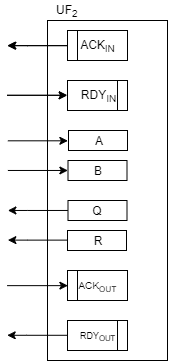
\includegraphics[scale=1]{transliv_es.png}
\columnbreak
\begin{center}
\begin{lstlisting}
0.  (RDYIN = 0) nop, 0
    (= 1)       A -> TA, B -> TB, set ACKIN,
                reset RDYIN, 1
1.  0 -> TQ, 2
2.  (segno(TA - TB), ACKOUT = 0-) TQ + 1 -> TQ,
                                  TA - TB -> TA, 2
    (= 11) TA -> R, TQ -> Q, set RDYOUT, reset ACKOUT ...
\end{lstlisting}
\end{center}
Possiamo notare che UF$_1$ manda i segnali A e B e \textbf{non ha altre operazioni mentre attende la risposta Q, R da UF$_2$}. Questa situazione si chiama \textbf{protocollo domanda/risposta} e solo in questo caso basta una coppia di indicatori di transizione.
\begin{center}
\begin{lstlisting}
UF1
0.  ... -> A, set RDY, 1
1.  (ACK = 0) nop, 1
    (= 1)     B -> ..., reset ACK

    
UF2
0.  (RDY = 0) nop, 0
    (= 1) A -> ..., 1
... elaborazione di UF2 ...
n.  ... -> B, set ACK, reset RDY, 0
\end{lstlisting}
\end{center}
\end{multicols}
\pagebreak
\subsection{Comunicazioni asincrone a n posizioni}
In questo caso \textbf{non esiste una soluzione basata su semplici interfacce nelle due unità comunicati}, ma è \textbf{necessario introdurre una terza unità} (chiamata \textbf{unità buffer}) che \textbf{implementi una coda FIFO a n posizioni}.\\
Il \textbf{mittente può spedire al più n messaggi senza che il destinatario effettui ricezioni}.
\begin{center}
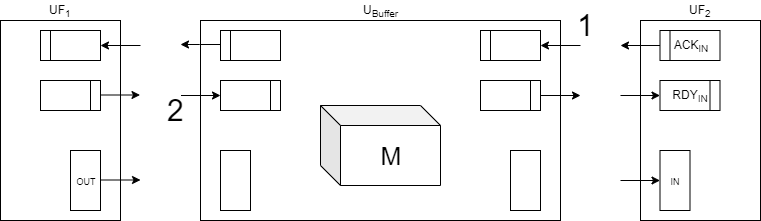
\includegraphics[scale=0.7]{asynnpos.png}
\end{center}
\paragraph{1} Se ci sono messaggi in memoria M, manda un messaggio a UF$_2$
\paragraph{2} Se c'è posto in memoria M, riceve un messaggio da UF$_1$ e lo memorizza in M
\paragraph{} Se valgono entrambe ed M è vuota, allora il messaggio in ingresso da UF$_1$ viene passato direttamente ad UF$_2$
\paragraph{U$_{buffer}$} Il codice di U$_{buffer}$ avrà come \textbf{variabili di condizionamento RDY da UF$_1$}, \textbf{ACK da UF$_2$}, \textbf{condizione di memoria piena} e \textbf{condizione di memoria vuota}.\\
Le due condizioni di memoria piena/vuota possono essere gestite tramite un semplice contatore. SE per esempio abbiamo una memoria M con 2$^k$ posizioni, useremo un contatore da k + 1 bit:
\begin{list}{}{}
	\item Memoria vuota \texttt{OR(CONT) = 0}
	\item Memoria piena \texttt{CONT$_0$ = 1}
\end{list}
$\Rightarrow$ \texttt{0. (RDY, ACK, OR(CONT), CONT$_0$, \ldots}\\\\
Il buffer implementa una politica \textbf{FIFO}: \textbf{il primo messaggio inviato} da UF$_1$ \textbf{deve essere il primo messaggio letto} da UF$_2$
\subsection{Comunicazioni asimmetriche}
\paragraph{BUS} Per poter parlare delle comunicazioni asimmetriche è necessario introdurre il concetto di BUS. Un \textbf{BUS è un insieme di linee per trasportare dati} (es. da 32 bit), \textbf{l'indirizzo} (es. log$_2$ n bit) \textbf{e una linea da 1 bit che indica l'operazione da svolgere}.
\begin{center}
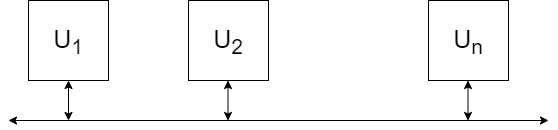
\includegraphics[scale=0.9]{bus.png}
\end{center}
\pagebreak
Il grosso svantaggio di questo tipo di comunicazione è che \textbf{le unità possono comunicare solamente una alla volta}. Ho bisogno quindi di un \textbf{meccanismo di arbitraggio} che regola l'ordine di comunicazione delle varie unità.\\
Vedremo due tipi di arbitraggio: \textbf{centralizzato} e \textbf{distribuito}.\\
Inoltre avremo a disposizione anche un protocollo d'interazione Unità --- BUS:\\richiesta da U$_i$ di uso del BUS $\rightarrow$ comunicazione (uso del BUS) $\rightarrow$ rilascio della risorsa.\\\\
Rimane da sottolineare il \textbf{problema della sincronizzazione}. Abbiamo bisogno di indicatori a livello per poter comunicare in maniera asimmetrica con un BUS.
\subsubsection{Arbitri Centralizzati}
\paragraph{Arbitro Centralizzato a Richieste Indipendenti} La unità hanno un \textbf{collegamento diretto con l'arbitro}
\begin{multicols}{2}
\begin{center}
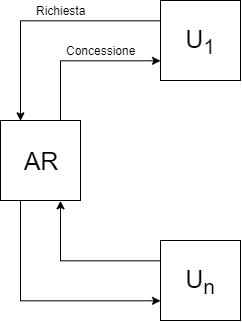
\includegraphics[scale=0.5]{arcentrrichind.png}
\end{center}
\columnbreak
L'arbitro AR \textbf{considera le richieste}, fra di esse \textbf{individura l'unità} U$_i$ vincitrice \textbf{secondo una certa politica} P e \textbf{assegna la richiesta} all'unità individuata. Dopodiché, attende il rilascio della risorsa assegnata.
\end{multicols}
\paragraph{Arbitro Centralizzato Daisy Chaining} Abbiamo un numero minore di ingressi ma la stessa politica del caso precedente.
\begin{center}
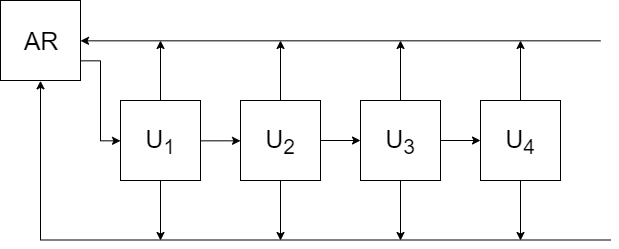
\includegraphics[scale=0.5]{arcentrdaisy.png}
\end{center}
Il vantaggio di questo arbitro è la sua semplicità: due ingressi ed una uscita.\\
L'arbitro, se c'è richiesta, manda il segnale di disponibilità alla prima unità. Il segnale viene passato da unità ad unità, finché non viene trovata l'unità che ne ha fatto richiesta. A tal punto, tale unità manda all'arbitro il bit di occupato, ed inizia ad utilizzare la risorsa. Infine, l'arbitro attende che il bit di occupato torni a 0.
\paragraph{Arbitro Centralizzato Polling} L'arbitro interroga le varie unità per sapere se hanno bisogno della risorsa BUS, ed assegna le risorse secondo una certa politica.
\paragraph{Aribtro Centralizzato a Divisione di Tempo} Questa soluzione consiste nell'assegnare l'accesso alla risorsa comune ad ogni unità U$_i$ per \textbf{istanti di tempo ben determinati}.
\pagebreak
\subsubsection{Arbitri Decentralizzati}
\paragraph{Arbitro Decentralizzato a Disciplina Circolare (Token Ring)}
\begin{center}
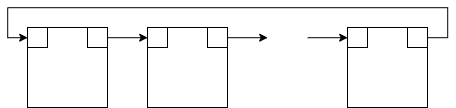
\includegraphics[scale=0.7]{ardectoken.png}
\end{center}
Se U$_i$ riceve 1 (token) in ingresso e deve utilizzare la risorsa allora la usa. In ogni caso, sia che debba utilizzarla sia che non debba farlo, passa il token in uscita alla prossima unità.
\paragraph{Non Deterministici} Usati soprattutto nelle reti wireless.
\begin{center}
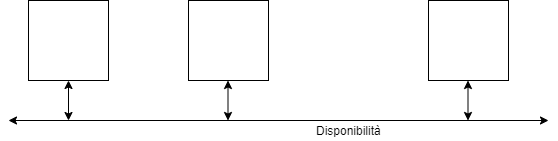
\includegraphics[scale=0.65]{arnondet.png}
\end{center}
In questa tipologia di arbitro può succedere che due o più unità rilevino la disponibilità e inizino a trasmettere \textbf{contemporaneamente}.\\
Tale problema viene risolto con \textbf{un sistema per rilevare le collisioni}: ogni unità che trasmette ascolta ciò che l'arbitro trasmette. Se ciò che ascolta è il medesimo segnale che ha inviato allora l'invio del messaggio è andato a buon fine, altrimenti se ascolta un messaggio differente allora aspetta un lasso di tempo casuale per poi ritentare la trasmissione.
\section{Memoria Modulare}
\pagebreak
\chapter{Macchina Assembler}
In questa parte andremo a vedere alcuni moduli che sono \textbf{unità firmware a tutti gli effetti}, con una \textbf{certa struttura di interconnessione} e che \textbf{riescono ad eseguire istruzioni assembler ASM}. In sostanza, \textbf{i processori}.
\begin{center}
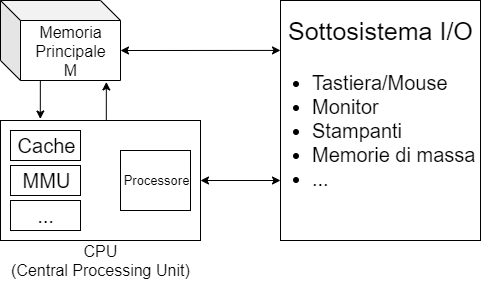
\includegraphics[scale=0.7]{macchinaassemblerschema.png}
\end{center}
\section{CPU}
\paragraph{Processore} Una \textbf{unità firmware in grado di eseguire operazioni esterne che sono istruzioni del linguaggio ASM}.
\paragraph{Cache} Una \textbf{memoria piccola ma molto veloce}, che \textbf{contiene il sottoinsieme della memoria principale M che permette di eseguire un certo programma}.
\paragraph{MMU} La \textbf{Memory Management Unit} è il \textbf{componente che permette di tradurre gli indirizzi logici} generati dal processore \textbf{in indirizzi fisici}
\paragraph{Logicamente} Dal punto di vista logico, un \textbf{processore P fa un ciclo infinito in cui legge l'istruzione all'indirizzo IC} (Instruction Counter) \textbf{o PC} (Program Counter), \textbf{la decodifica} e \textbf{la esegue}, poi \textbf{aggiorna IC e gestisce le interruzioni} (eventi \textbf{generati dal sottosistema I/O})
\begin{center}
\begin{lstlisting}
while(true) {
	FETCH	;legge istruzione a indirizzo IC/PC
	DECODE	;decodifica istruzione
	EXECUTE	;esegue istruzione
		;aggiorna IC/PC
	INT	;gestisci interruzioni/eccezioni
}
\end{lstlisting}
\end{center}
\pagebreak
\section{Istruzioni ASM}
\paragraph{Dati} Le istruzioni assembler (ASM) operano sostanzialmente su \textbf{due tipi di dato}:
\begin{list}{}{}
	\item \textbf{Registri Generali} RG: \textbf{pochi}, \textbf{velocissimi}, lunghi una parola, a doppia porta (permettono di leggere due locazioni e scrivere una locazione nello stesso ciclo di clock)
	\item \textbf{Locazioni di memoria}: \textbf{molte}, \textbf{lente}, lunghe una parola, \textbf{esterne al processore} che interagisce con M tramite un meccanismo domanda/risposta.
\end{list}
\paragraph{Istruzioni} I tipi di istruzioni presenti sono:
\begin{list}{}{}
	\item \textbf{Operative}: somma, shift\ldots
	\item \textbf{Accesso} alla memoria: lettura (M $\rightarrow$ RG) o scrittura (RG $\rightarrow$ M)
	\item \textbf{Salto Condizionale}, con condizione sui RG
	\item \textbf{Salto Incondizionale}
\end{list}
\section{Programmi e processi}
Assumeremo che \textbf{ogni programma ASM veda uno Spazio di Indirizzamento detto Memoria Virtuale} (MV), schematizzato di seguito.
\begin{multicols}{2}
\paragraph{MV} La \textbf{memoria virtuale} la vediamo come un \textbf{vettore} le cui \textbf{posizioni vanno da un indirizzo 0 ad un indirizzo MAX} (indirizzi logici), ognuno dei quali corrisponde ad \textbf{una parola} (32/64 bit).\\
Lo spazio viene organizzato secondo lo schema a fianco.
\columnbreak
\begin{center}
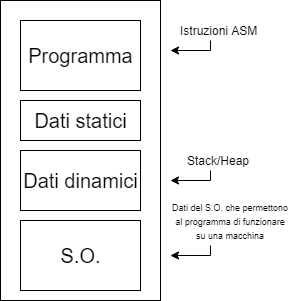
\includegraphics[scale=0.6]{progproc.png}
\end{center}
\end{multicols}
\paragraph{Da programma a processo} Quando un \textbf{programma entra in esecuzione diventa un processo}. Di seguito uno schema che racconta le fasi di un programma C che diventa un processo.
\begin{center}
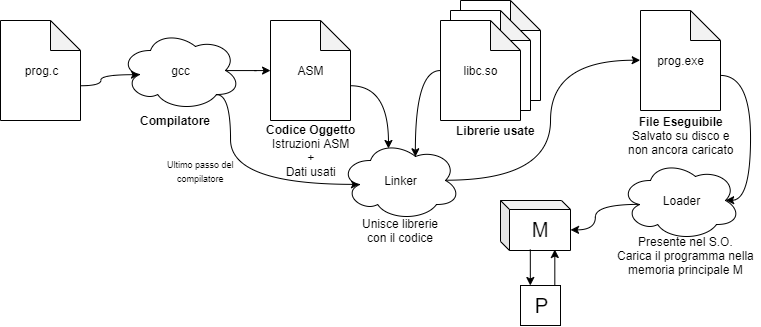
\includegraphics[scale=0.6]{prog2proc.png}
\end{center}
\pagebreak
\section{Spazio di Indirizzamento Logico e Memoria Virtuale}
\paragraph{Indirizzi} Gli \textbf{indirizzi generati} dal processore, durante l'esecuzione di un processo, \textbf{non sono indirizzi della memoria principale} -- cioè \textbf{indirizzi fisici} -- ma \textbf{indirizzi logici} cioè \textbf{riferiti ad un'astrazione della memoria del processo detta Memoria Virtuale} (MV).\\
L'\textbf{insieme degli indirizzi logici di un processo è detto Spazio Logico di Indirizzamento}.\\
Il codice eseguibile del processo/programma, generato dal compilatore, è quindi riferito alla MV, ed il processore genera \textbf{indirizzi logici sia per il codice che per i dati}.
\paragraph{Rilocazione} Quando un processo viene \textbf{creato e caricato}, ad esso viene \textbf{allocata una porzione della memoria principale} la cui \textbf{ampiezza} e i cui \textbf{indirizzi non coincidono con quelli della MV} del processo, ma viene \textbf{stabilita una corrispondenza tra indirizzi logici} della MV \textbf{e indirizzi fisici} della M. Questa funzione, detta \textbf{funzione di rilocazione o traduzione} dell'indirizzo, è \textbf{implementata come una tabella associata al processo della Tabella di Rilocazione}.\\
Il processo di traduzione deve essere \textbf{molto veloce} ed è eseguito dalla \textbf{MMU} (Memory Management Unit).
\subsection{Modalità di Indirizzamento}
Vediamo come esprimere la locazione di un certo operando di un'istruzione ASM. Supponiamo di avere l'istruzione \texttt{INC X}, che incrementa un valore intero. Vediamo la \texttt{X} prima come un RG e poi come una M.
\begin{multicols}{2}
\paragraph{Registro} \texttt{RG[4]}, \texttt{R4}
\begin{center}
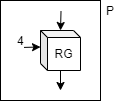
\includegraphics[scale=1]{indiriz_rg.png}
\end{center}
\columnbreak
\paragraph{Locazione di memoria} Ci sono diversi modi per esprimerlo:
\begin{list}{}{}
	\item \textbf{Assoluto}\\R$_i$ $\Rightarrow$ \texttt{M[RG[i]]}
	\item \textbf{Base + indice}\\R$_i$(R$_s$) $\Rightarrow$ \texttt{M[RG[i] + RG[s]]}
	\item \textbf{Relativo} ad IC/PC\\R$_i$ $\Rightarrow$ \texttt{M[IC + RG[i]]}
\end{list}
\end{multicols}
Le modalità di indirizzamento \textbf{registro} e \textbf{locazione assoluta} sono \textbf{molto simili}: la differenza sta in come si usa il registro, nel primo caso direttamente come dato e nel secondo come indirizzo di memoria.
\begin{center}
\begin{tabular}{c | c}
\textbf{Istruzioni ASM} & \textbf{Operandi} \\
\hline
Operative & Registro \\
Memoria & Base + Indice \\
Stato & Assoluto/Relativo
\end{tabular}
\end{center}
\section{RISC vs CISC}
\paragraph{RISC} \textbf{Reduced} Instruction Set Computer
\paragraph{CISC} \textbf{Complex} Instruction Set Computer
\paragraph{Dilemma} Il progettista dell'architettura di un calcolatore si è sempre trovato di fronte al dilemma "\textit{set di istruzioni semplici}" (RISC) oppure "\textit{set di istruzioni complesse}" (RISC). L'esigenza di avere un set di istruzioni complesso nasce dal desiderio di avere una \textbf{corrispondenza il più possibile uno-a-uno tra le istruzioni della macchina ASM e i comandi e le strutture dati dei linguaggi ad alto livello}.\\
In linea di principio, l'approccio CISC dovrebbe \textbf{comportare un aumento di prestazioni rispetto al RISC}, in quanto, a parità di computazione, \textbf{ciò che in RISC viene espresso con una sequenza molto lunga di istruzioni ASM}, \textbf{in CISC è espresso con poche istruzioni}.
\paragraph{Vantaggi e Svantaggi} Molti dei vantaggi potenziali ottenibili con l'approccio CISC si sono rilevati meno ovvi di quanto sembri a prima vista, talvolta addirittura tramutandosi in svantaggi. Infatti \textbf{la complessità delle istruzioni e dei modi di indirizzamento può aumentare la lunghezza delle parole dell'istruzione e il numero di accessi in memoria}.\\
Stabilire il migliore è impossibile, ma a livello didattico conviene studiare l'approccio RISC, in particolare il D-RISC.
\pagebreak
\chapter{D-RISC}
Il \textbf{Didactic-Reduced Instruction Set Computer} è un \textbf{assembler didattico di tipo RISC}. Le sue caratteristiche sono le seguenti.
\subparagraph{Registri Generali} Sono presenti \textbf{64 registri general purpose} (\texttt{RG[0 .. 63]}), cioè in cui posso scrivere qualsiasi cosa, \textbf{da 32 bit}.\\
Il registro R$_0$ è \textbf{particolare} e \textbf{contiene sempre 0 al proprio interno}.
\subparagraph{Parole} Le parole all'interno dei registri \textbf{sono da 32 bit}.\\
Questa caratteristica non è vincolante, anche avendo parole da 64 bit la struttura della macchina non cambia.
\subparagraph{Istruzioni D-RISC} In generale il D-RISC contiene \textbf{questo set di istruzioni}:
\begin{list}{}{}
	\item \textbf{Operative}: operazioni artimetico-logiche fra registri
	\item \textbf{Load/Store}: caricano dati da/in memoria
	\item \textbf{Salto} condizionato/incondizionato
\end{list}
Delle istruzioni si vedranno sintassi e formato in memoria, cioè come vengono rappresentate mediante parole da 32 bit.
\subparagraph{Memoria} La \textbf{memoria principale è indirizzabile alla parola}.
\section{Istruzioni}
\subsection{Operative}
Comprendono le istruzioni aritmetiche su interi e logiche più comuni. Sono \textbf{tutte registro--registro}.
\subparagraph{Con Operandi e risultato in RG} \texttt{ADD op1, op2, op3}\\
Es. \texttt{ADD R$_5$, R$_{27}$, R$_3$}, semantica: \texttt{R[5] + R[27] $\rightarrow$ R[3]}.\\
In memoria: \begin{tabular}{| c | c | c | c | c |}
\hline
8 bit & 6 bit & 6 bit & 6 bit & 6 bit \\
\hline
ADD & R$_5$ & R$_{27}$ & R$_3$ & \\
\texttt{CODOP} & \texttt{op1} & \texttt{op2} & \texttt{op3} & \\
\hline
\end{tabular}
\subparagraph{Con uno dei due operandi immediato} \texttt{ADDI op1, op2, op3}\\
Es. \texttt{ADDI R$_5$, \#8, R$_{27}$}, semantica: \texttt{R[5] + 8 $\rightarrow$ R[27]}\\
In memoria: \begin{tabular}{| c | c | c | c |}
\hline
8 bit & 6 bit & 6 bit & 12 bit \\
\hline
ADD & R$_5$ & R$_{27}$ & \textit{costante in comp. a 2} \\
\hline
\end{tabular}
\paragraph{} Questi tipi di operazioni posso farle con \texttt{ADD}, \texttt{SUB}, \texttt{MUL}, \texttt{DIV}, \texttt{SHR}, \texttt{SHL}.
\subparagraph{Istruzioni logiche} \texttt{AND}, \texttt{OR} e \texttt{NOT}\\
Esempio: \texttt{AND R$_1$, R$_2$, R$_3$}, semantica \texttt{R[1] AND R[2] $\rightarrow$ R[3]}\\
In memoria: \begin{tabular}{| c | c | c | c | c |}
\hline
8 bit & 6 bit & 6 bit & 6 bit & 6 bit\\
\hline
AND & R$_1$ & R$_2$ & R$_3$  & \\
\hline
\end{tabular}
\pagebreak
\subsection{Load/Store}
Non sono singole $\mu$-istruzioni perchè c'è una comunicazione tra UF (processore--memoria). Sono le \textbf{uniche istruzioni memoria--registro del D-RISC}. Come visto in precedenza, l'\textbf{indirizzo logico in memoria è calcolato come somma del contenuto di due registri generali}, uno che funge da \textbf{base} e uno da \textbf{indice}.
\begin{multicols}{2}
\begin{center}
\textbf{Sintassi}\\
\texttt{LOAD R$_B$, R$_i$, R$_X$}\\
\texttt{STORE R$_B$, R$_i$, R$_X$}
\end{center}
\columnbreak
\begin{center}
\textbf{Semantica}\\
\texttt{M[R[B] + R[i]] $\rightarrow$ R[X]}\\
\texttt{R[X] $\rightarrow$ M[R[B] + R[i]]}
\end{center}
\end{multicols}
\begin{center}
\textbf{In memoria} (analogo per entrambe):  
\begin{tabular}{| c | c | c | c | c |}
\hline
8 bit & 6 bit & 6 bit & 6 bit & 6 bit\\
\hline
LOAD/STORE & R$_B$ & R$_i$ & R$_X$  & \\
\hline
\end{tabular}
\end{center}
Inoltre, possiamo avere un'\textbf{ulteriore istruzione che realizza lo scambio del contenuto tra una locazione di memoria e un RG}.

\begin{multicols}{2}
\begin{center}
\textbf{Sintassi}\\
\texttt{EXCHANGE R$_B$, R$_i$, R$_X$}
\end{center}
\columnbreak
\begin{center}
\textbf{Semantica}\\
\texttt{M[R[B] + R[i]] $\leftrightarrow$ R[X]}
\end{center}
\end{multicols}
\begin{center}
\textbf{In memoria}:  
\begin{tabular}{| c | c | c | c | c |}
\hline
8 bit & 6 bit & 6 bit & 6 bit & 6 bit\\
\hline
EXCHANGE & R$_B$ & R$_i$ & R$_X$  & \\
\hline
\end{tabular}
\end{center}
\subsection{Salto Condizionato}
Permettono di \textbf{saltare un numero preciso di istruzioni} a seconda della condizione imposta.
\subparagraph{Confronto fra due RG} Usando gli operatori logici $>$, $<$, $=$, $\neq$, $\leq$, $\geq$\\
Sintassi, esempio con $>$: \texttt{IF$_>$, R$_i$, R$_s$, offset}\\
Semantica: se \texttt{R[i] $>$ R[s]} allora \texttt{IC + offset $\rightarrow$ IC}, altrimenti \texttt{IC + 1 $\rightarrow$ IC}.\\
\textbf{In memoria}:  
\begin{tabular}{| c | c | c | c |}
\hline
8 bit & 6 bit & 6 bit & 12 bit \\
\hline
IF$_>$ & R$_i$ & R$_s$ & offset \\
\hline
\end{tabular}
\subparagraph{Confronto fra un RG e una costante} Sempre usando gli operatori logici.\\
Sintassi, esempio con $>$: \texttt{IF$_{> 0}$, R$_i$, offset}\\
Semantica: se \texttt{R[i] $>$ 0} allora \texttt{IC + offset $\rightarrow$ IC}, altrimenti \texttt{IC + 1 $\rightarrow$ IC}.\\
\textbf{In memoria}:  
\begin{tabular}{| c | c | c |}
\hline
8 bit & 6 bit & 18 bit \\
\hline
IF$_{> 0}$ & R$_i$ & offset \\
\hline
\end{tabular}
\subsection{Salto Incodizionato}
Permettono di \textbf{saltare un numero preciso di istruzioni} senza valutare nessuna condizione.
\subparagraph{Salto con offset} \texttt{GOTO offset}\\
Semantica: \texttt{IC + offset $\rightarrow$ IC}\\
\textbf{In memoria}:  
\begin{tabular}{| c | c |}
\hline
8 bit & 24 bit \\
\hline
GOTO & offset \\
\hline
\end{tabular}
\subparagraph{Salto con RG} \texttt{GOTO R$_i$}\\
Semantica: \texttt{IC + R[i] $\rightarrow$ IC}\\
\textbf{Non c'è lo stack}, quindi è impossibile la ricorsione.
\subparagraph{Chiamata a procedura} \texttt{CALL R$_F$, R$_{RET}$}
\begin{list}{}{}
	\item R$_F$: indirizzo della funzione/procedura
	\item R$_{RET}$: indirizzo di ritorno all'uscita
\end{list}
Semantica: \texttt{R[F] $\rightarrow$ IC, IC + 1 $\rightarrow$ R[RET]}, operazioni fatte in contemporanea.\\
Solo per procedure non ricorsive!
\pagebreak
\section{Compilazione}
Vediamo una serie di esempi su come si compilano alcuni comandi presi dal linguaggio C.
\paragraph{Assegnamento}
\begin{multicols}{2}
\begin{center}
	\begin{C}
	int x;
	x = 0;
	x = 123;
	x = z;
	\end{C}
	\begin{C}
	int y[16];
	y[8] = 0;
	x = y[8];
	\end{C}
\end{center}
\columnbreak
\begin{center}
	\begin{lstlisting}
	Rx
	ADD R0, R0, Rx
	ADDI R0, #123, Rx
	;Possibile, 123 < 2^12
	ADD Rz, R0, Rx
	\end{lstlisting}
	\begin{lstlisting}
	Rby
	;Indirizzo di partenza del vettore
	STORE Rby, #8, R0
	LOAD Rby, #8, Rx
	\end{lstlisting}
\end{center}
\end{multicols}
\paragraph{Diramazione Condizionale}
\begin{multicols}{2}
\begin{center}
	\begin{C}
	if (e) {
		//body
	}
	\end{C}
	\begin{C}
	if (x == 0) {
		y = y + 1;
	}
	\end{C}
\end{center}
\columnbreak
\begin{center}
	\begin{lstlisting}
		IF not(e), cont
		;compilazione body
	cont:	;resto del programma
	\end{lstlisting}
	\begin{lstlisting}
		IF!=0 Rx, cont
		ADDI Rx, #1, Ry
	cont:	;resto del programma
	\end{lstlisting}
\end{center}
\end{multicols}
\paragraph{Diramazione Condizionale con else}
\begin{multicols}{2}
\begin{center}
	\begin{C}
	if (e) {
		//body then
	} else {
		//body else
	}
	\end{C}
	\begin{C}
	if (x == 0) {
		y = y + 1;
	} else {
		y = x - 1;
	}
	\end{C}
\end{center}
\columnbreak
\begin{center}
	\begin{lstlisting}
		IF e, then
		;compilazione body else
		GOTO cont
	then:	;compilazione body then
	cont:	;resto del programma
	\end{lstlisting}
	\begin{lstlisting}
		IF=0 Rx, then
		SUB Rx, #1, Ry
		GOTO cont
	then:	ADD Rx, #1, Ry
	cont:	;resto del programma
	\end{lstlisting}
\end{center}
\end{multicols}
\pagebreak
\paragraph{Ciclo Indeterminato}
\begin{multicols}{2}
\begin{center}
	\begin{C}
	while (e) {
		//body
	}
	\end{C}
	\begin{C}
	while (x < n) {
		y = y + x;
		x = x * 2;
	}
	\end{C}
\end{center}
\columnbreak
\begin{center}
	\begin{lstlisting}
	while:	IF not(e), cont
		;compilazione body
		GOTO while
	cont:	;resto del programma
	\end{lstlisting}
	\begin{lstlisting}
	while:	IF>= Rx, Rn, cont
		ADD Ry, Rx, Ry
		MUL Rx, #2, Rx
		GOTO while
	cont:	;resto del programma
	\end{lstlisting}
\end{center}
\end{multicols}
\paragraph{Ciclo Determinato}
\begin{multicols}{2}
\begin{center}
	\begin{C}
	for (iniz; cond; incr) {
		//body
	}
	\end{C}
	\begin{C}
	for (i = 0; i < n; i++) {
		x[i] = 0;
	}
	\end{C}
\end{center}
\columnbreak
\begin{center}
	\begin{lstlisting}
	;assumo di fare almeno un'iterazione
		;compilazione iniz
	for:	;compilazione body
		;compilazione incr
		IF cond, for
	cont:	;resto del programma
	\end{lstlisting}
	\begin{lstlisting}
	for:	STORE Rbx, Ri, R0
		ADD Ri, #1, Ri
		IF< Ri, Rn, for
	cont:	;resto del programma
	\end{lstlisting}
	Si può ottimizzare con la \textbf{tecnica dell'unrolling}: se n è pari, posso fare cicli con \texttt{i += 2}, se è multiplo di 10 con \texttt{i += 10}\ldots
\end{center}
\end{multicols}
\paragraph{Prodotto fra vettori}
\begin{multicols}{2}
\begin{center}
	\begin{C}
	sum = 0;
	for (i = 0; i < n; i++) {
		sum += x[i] * y[i]
	}
	\end{C}
\end{center}
\columnbreak
\begin{center}
	\begin{lstlisting}
		ADD R0, R0, Rsum
		ADD R0, R0, Ri
	for:	LOAD Rbx, Ri, Rxi
		LOAD Rby, Ri, Ryi
		MUL Rxi, Ryi, Rmul
		ADD Rsum, Rmul, Rsum
		ADD Ri, #1, Ri
		IF< Ri, Rn, for
	\end{lstlisting}
\end{center}
\end{multicols}
\pagebreak
\section{Processore come UF}
Vediamo come \textbf{schematizzare un processore} (P) \textbf{come una generica Unità Firmware}.
\paragraph{DMA} \textbf{Direct Memory Access}, BUS che consente alle unità di I/O di \textbf{comunicare direttamente con la memoria M}.
\begin{center}
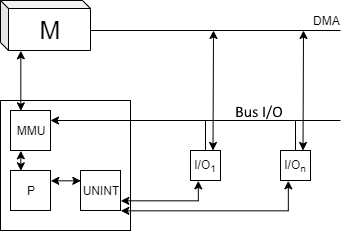
\includegraphics[scale=1]{procuf.png}
\end{center}
\paragraph{Processore} Possiamo definire un processore come un'\textbf{unità firmware che esegue un ciclo infinito in cui si eseguono le operazioni esterne}. Le operazioni del processore possono essere descritte, in un linguaggio più "informatico", come segue:
\begin{C}
while(true) {
	fetch ISTR (IC/PC) //LOAD di una istr, ricordiamo che PC=IC stessa cosa
	decode ISTR
	exec ISTR
	trattamento interruzioni
}
\end{C}
Che diventa l'\textbf{interprete ASM in $\mu$-codice a livello firmware}.\\
Un processore può essere semplicisticamente schematizzato come segue:
\begin{center}
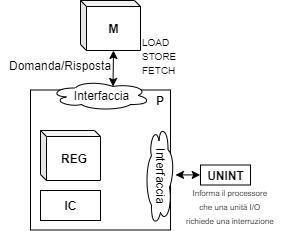
\includegraphics[scale=1]{procschema.png}
\end{center}
\pagebreak
\subsection{Interfaccia verso la memoria}
Di seguito lo schema dell'\textbf{interfaccia a transizione di livello del processore verso la memoria} su collegamenti dedicati.
\begin{center}
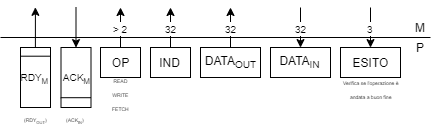
\includegraphics[scale=1.2]{interfaccia_pm.png}
\end{center}
Su altre fonti possiamo trovare due coppie di sincronizzatori (ACK e RDY), ma si assume che l'interfaccia sia a domanda/risposta, quindi possiamo usare una coppia sola.
\subsection{Interfaccia verso UNINT}
Di seguito lo schema dell'\textbf{interfaccia del processore verso l'unità UNINT}.
\begin{multicols}{2}
\begin{center}
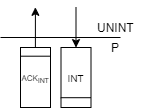
\includegraphics[scale=1.2]{interfaccia_punint.png}
\end{center}
\columnbreak
Se \textbf{durante l'esecuzione} del ciclo infinito \textbf{si riceve\\INT = 1}, allora \textbf{il processore deve trattare l'interruzione}: \textbf{manda ACK$_{INT}$} e \textbf{fa due LOAD} per ottenere il numero di unità I/O che ha richiesto l'interruzione e il motivo. Successivamente \textbf{invoca il driver corretto per il dispositivo}.
\end{multicols}
\pagebreak
\section{Interprete Firmware}
Scriviamo una prima versione dell'interprete firmware con il $\mu$-linguaggio, un estratto:
\begin{lstlisting}
0.	fetch -> OP, IC -> IND, set RDYM, 1

1.	(ACKM, OR(ESITO) = 0-) nop, 1
	(= 10) DATAIN -> IR, reset ACKM, 2
	;                ^^ IR = Instruction Register
	(= 11) ..., trattecc
	;           ^^^^^^^^ Trattamento eccezioni

2.	(IR.CODOP, INT = "ADD", 0) R[IR.RA] + R[IR.RB] -> R[IR.RC], IC + 1 -> IC, 0
	(= "ADD", 1) R[IR.RA] + R[IR.RB] -> R[IR.RC], IC + 1 -> IC, trattint
	;                                  Trattamento interruzioni ^^^^^^^^
	(= "LOAD", 0) read -> OP, R[IR.RA] + R[IR.RB] -> IND, set RDYM, reset ACKM, 3
	(= "IF<", 0) segno(R[IR.RA] - R[IR.RB]) -> S, 4
	...

3.	(ACKM, OR(ESITO), INT = 0--) nop, 3
	(= 100) DATAIN -> R[IR.RC], reset ACKM, IC + 1 -> IC, 0
	(= 101) DATAIN -> R[IR.RC], reset ACKM, IC + 1 -> IC, trattint
	(= 110) ..., trattecc
	
4.	(S, INT = 10) IC + IR.offset -> IC, 0
	(= 11) IC + IR.offset -> IC, trattint
	(= 00) IC + 1 -> IC, 0
	(= 01) IC + 1 -> IC, trattint
...
\end{lstlisting}
\paragraph{IR} L'\textbf{Instruction Register} è da intendersi come un \textbf{registro interno}, cioè non d'interfaccia. In questo registro andiamo a \textbf{memorizzare tutti i bit che ci indicano l'istruzione da eseguire}.\\
Con \texttt{IR.CODOP} o \texttt{IR.RB} si intendono \textbf{i soli bit che indicano il codice operativo} (operazione), i \textbf{registri} o l'\textbf{etichetta per i salti}.
\paragraph{Problema} Il problema di questa prima versione dell'interprete firmware \textbf{riguarda la decodifica del Codice Operativo} che ogni volta viene mandato alla PC del processore per gestire i vari $\alpha$, $\beta$ della PO in modo da eseguire le operazioni corrette.\\
Essendo il codice operativo un \textbf{frammento di 8 bit}, possiamo avere \textbf{una $\mu$-istruzione con ben 256 frasi alternative} che comporta un \textbf{esponenziale aumento di complessità di progettazione}.
\paragraph{Soluzione} La soluzione al problema è quella di \textbf{avere una $\mu$-istruzione che usa il codice operativo per dire al processore di andare ad eseguire quella istruzione} di $mu$-codice \textbf{che ha come indirizzo il valore del codice operativo}.\\
Quindi il codice operativo viene mandato alla PC, che \textbf{decide quale sarà il suo stato interno} (e quindi \textbf{la prossima $\mu$-istruzione}) durante il prossimo ciclo di clock. Questa tecnica si chiama \textbf{Salto Forzato}, simile per principio al controllo residuo.\\\\
A pagina seguente il codice che sfrutta questa tecnica. Notare l'evidente ottimizzazione.
\pagebreak
\begin{lstlisting}
fch0.	fetch -> OP, IC -> IND, set RDYM, fch1

fch1.	(ACKM, OR(ESITO) = 0-) nop, fch1
	(= 10) DATAIN -> IR, DATAIN.COP -> RC ;decido la prossima istruzione
	
add0.	(INT = 0) R[IR.RA] + R[IR.RB] -> R[IR.RC], IC + 1 -> IC, fch0
	(= 1) R[IR.RA] + R[IR.RB] -> R[IR.RC], IC + 1 -> IC, trattint

load0.	read -> OP, R[IR.RA] + R[IR.RB] -> IND, set RDYM, load1

load1.	(ACKM, OR(ESITO), INT = 0--) nop, load1
	(= 100) DATAIN -> R[IR.RC], IC + 1 -> IC, fch0
	(= 101) DATAIN -> R[IR.RC], IC + 1 -> IC, trattint
	(= 110) ..., trattecc
	
if<0.	segno(R[IR.RA] - R[IR.RB]) -> S, if<1

if<1.	(S, INT = 10) IC + IR.offset -> IC, fch0
	(= 11) IC + IR.offset -> IC, trattint
	(= 00) IC + 1 -> IC, fch0
	(= 01) IC + 1 -> IC, trattint
\end{lstlisting}
In questa versione abbiamo almeno \textbf{una istruzione in $\mu$-codice per ogni istruzione ASM}.\\
Si può notare che la decisione di quale $\mu$-istruzione eseguire è \textbf{determininata da \texttt{DATAIN.COP -> RC}}, \textbf{dove andiamo a scrivere gli 8 bit che determinano il codice operativo} dell'istruzione ASM \textbf{direttamente nel registro di stato della PC (RC)}, in modo da determinare quale $\mu$-istruzione eseguire immediatamente dopo.
\subsection{Valutazione delle prestazioni}
Il \textbf{tempo effettivo di accesso in memoria t$_a$} è \textbf{maggiore del ciclo di clock del processore}: per questo è uno dei principali problemi da risolvere per il raggiungimento di prestazioni elevate.
\begin{center}
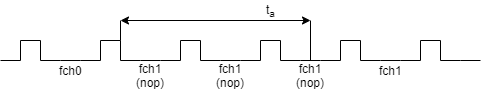
\includegraphics[scale=1]{valprest.png}
\end{center}
\begin{multicols}{2}
Con il $\mu$-programma visto prima, siamo in grado di dare una valutazione del tempo di elaborazione per le istruzioni che caratterizzano il processore:
\begin{list}{}{}
	\item t$_{fch0}$ + t$_{fch1}$ = 2$\tau$ + t$_a$ \textbf{chiamata e decodifica}
	\item t$_{add}$ = t$_{sub}$ = 1$\tau$
	\item t$_{saltocond}$ = 2$\tau$
	\item t$_{saltoincd}$ = 1$\tau$
	\item t$_{load}$ = 2$\tau$ + t$_a$
	\item t$_{store}$ = 3$\tau$ + t$_a$
	\item t$_{mul}$ = t$_{div}$ = 50$\tau$ per convenzione
\end{list}
t$_a$ = 2($\tau$ + t$_{tr}$) + $\tau_m$ = 72$\tau$ accesso alla memoria molto lento.\\

\columnbreak
Tempo medio di elaborazione T, con formula vista in precedenza \texttt{$T = \tau * \sum_{i = 0}^{n - 1}(p_i * k_i) $}\\
Le probabilità come seguono:
\begin{list}{}{}
	\item Aritm-Logiche corte 40\%
	\item Aritm-Logiche lunghe 10\%
	\item Load/Store 30\%
	\item Salto 20\%
\end{list}
Inoltre le prestazioni variano anche in relazione al tipo di RAM: l'accesso a memorie dinamiche costa 60--100$\tau$, mentre a quelle statiche costa 20--40$\tau$
\end{multicols}
\pagebreak
\chapter{Superamento dei Limiti del Processore Monolitico}
Nel processore visto fin'ora come un'\textbf{unica struttura firmware} troviamo \textbf{due problemi essenziali}: il lungo tempo di accesso alla memoria e il lungo tempo di esecuzione delle istruzioni.
\paragraph{Tempo di Accesso alla Memoria} Una soluzione al problema consiste nell'\textbf{introdurre un ulteriore livello di gerarchia di memoria} tra la memoria principale ed i registri generali.\\
Tale memoria, detta \textbf{memoria cache}, è \textbf{molto piccola}, \textbf{molto veloce} ma anche \textbf{molto costosa} da realizzare. La cache \textbf{conterrà un sottoinsieme delle locazioni della memoria principale}.
\paragraph{Tempo di Esecuzione delle Istruzioni} Nel processore monolitico le varie operazioni da compiere (fetch, decode, operandi, execute, int) vengono \textbf{eseguite sequenzialmente una alla volta}. Possiamo \textbf{ottimizzare} questo comportamento \textbf{in due modi}:
\begin{list}{}{}
	\item \textbf{Processori Pipeline} o \textbf{a catena di montaggio}. Si caratterizzano per il \textbf{parallelismo nell'interprete firmware}, cioè \textbf{avere più UF che lavorano in parallelo}, ognuna con un particolare compito.
	\begin{multicols}{2}
	Spenderò tempo inizialmente per \textbf{riempire la catena di montaggio} (2$\tau$ per comunicare tra le UF), ma dopo un certo tempo \textbf{produrrà risultati in un tempo sicuramente inferiore} rispetto al processore monolitico.
	\begin{center}
		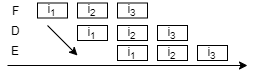
\includegraphics[scale=1]{pipeline.png}
	\end{center}
	\end{multicols}
	\item \textbf{Processori Superscalari}. Il concetto alla base è di \textbf{avere più processori che lavorano in simultanea} avendo una \textbf{memoria di registri in comune}.
\end{list}
\section{Gerarchie di Memoria}
\paragraph{Idea} Il concetto di gerarchie di memoria è \textbf{centrale alla strutturazione dei sistemi} ad un qualunque livello di astrazione.\\
All'interno di uno stesso elaboratore esistono vari tipi di memoria con caratteristiche molto diverse tra loro, quindi esiste una \textbf{gerarchia di memoria} nella quale al \textbf{livello più alto} stanno i \textbf{dispositivi di memoria più capaci}, più \textbf{lenti} e \textbf{meno costosi}, mentre man mano che \textbf{si scende di livello} i supporti hanno \textbf{capacità sempre più piccola}, \textbf{tempo di accesso inferiore} e \textbf{costo per bit maggiore}.\\\\
In termini di ottimizzazione del rapporto prestazioni/costo, l'obiettivo è di raggiungere \textbf{prestazioni paragonabili} (appena inferiori) a quelle che avremo se \textbf{tutta la massa di informazioni del sistema fosse concentrata nel solo livello inferiore}, e ad un \textbf{costo paragonabile} (appena superiore) a quello che avremmo se \textbf{tutta la massa di informazioni del sistema fosse concentrata nel solo livello più alto}.
\pagebreak
\subsection{Paginazione}
\paragraph{Memoria Virtuale -- Memoria Principale} Ritorniamo al concetto di memoria virtuale di un processo mandato in esecuzione ed ampliamo i concetti usati.
\begin{multicols}{2}
\begin{center}
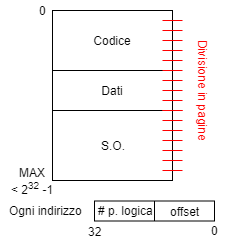
\includegraphics[scale=1]{paging.png}
\end{center}
Ogni \textbf{indirizzo logico} è \textbf{diviso in due parti}:
\begin{list}{}{}
	\item pochi bit indicano l'\textbf{offset}
	\item i restanti indicano il numero di pagina logica
\end{list}
In questo modo \textbf{suddividiamo la MV in pagine tutte della medesima dimensione}, indirizzate dall'offset.\\
Tale meccanismo è \textbf{molto utile per la traduzione} di indirizzi logici in fisici. In particolar modo quando in memoria principale vengono caricati più processi con dimensioni differenti e con tempi di esecuzione differenti. Spesso accade che un processo viene \textbf{caricato in memoria in maniera frammentaria} (cioè non è detto che gli indirizzi i e i+1 corrispondano agli indirizzi fisici s e s+1). Quindi avere un ulteriore metodo per raggruppare gli indirizzi è molto comodo.
\end{multicols}
\paragraph{Tabella di rilocazione} Ogni processo ha quindi una \textbf{tabella di rilocazione} che \textbf{associa ad ogni numero di pagina logica il numero di pagina fisica corrispondente}.\\
Ogni riga della tabella è una parola di 32 bit, usati per indicare la pagina fisica, ed 1 bit per indicare se è stata caricata o no.
\paragraph{Tipologie} La paginazione può essere:
\begin{list}{}{}
	\item \textbf{Statica}: carico tutte le pagine del processo in memoria e \textbf{ogni posizione rimane tale finché il processo è in esecuzione}
	\item \textbf{Dinamica}: carico tutte le pagine del processo in memoria, ma \textbf{può capitare che alcune pagine vengano scaricate} -- cioè messe in memoria secondaria -- \textbf{e ricaricate successivamente}. Questo metodo permette di caricare \textbf{solo le pagine utili all'esecuzione} del processo, quindi di \textbf{ottimizzare l'uso della memoria principale}.\\
	La paginazione dinamica ha due proprietà su cui basa la propria efficacia:
	\begin{list}{}{}
		\item \textbf{Località}: se al tempo t accedo a indx è molto probabile che al tempo t' non lontano da t acceda anche a indx+k con k piccolo.
		\item \textbf{Riuso}: se al tempo t accedo a indx è probabile che in un istante t' non lontano da t acceda nuovamente a indx.
	\end{list}
\end{list}
\subsubsection{Working Set}
Con \textbf{working set} si intende l'\textbf{insieme delle pagine che permettono l'esecuzione del programma in un certo istante alla massima velocità minimizzando il numero di fault}, ovvero senza dover portare in memoria principale altre pagine che si trovano in memoria secondaria.
\pagebreak
\subsubsection{Dimensione della pagina}
Adesso non resta che da capire quanto devono essere grandi le pagine. Partiamo da alcune semplici osservazioni:
\subparagraph{Pagine Piccole} $\Rightarrow$ Tante pagine
\subparagraph{Dimensione pagina}
\begin{list}{}{}
	\item \textbf{cresce} $\Rightarrow$ diminuisce la probabilità di informazioni che probabilmente accederò fra un po' in memoria
	\item \textbf{decresce} $\Rightarrow$ aumenta la probabilità che fra un po' mi serva un altra pagina
\end{list}
\paragraph{Fault di pagina} Il \textbf{pagefault} è il \textbf{tentativo di accedere ad un indirizzo non presente in memoria principale}.
\begin{multicols}{2}
\begin{center}
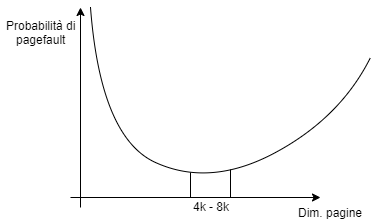
\includegraphics[scale=0.65]{pagefaultplot.png}
\end{center}
Dopo un certo limite le probabilità di fault tornano a crescere poiché con \textbf{pagine troppo grandi può accadere che per caricare nuove pagine vada a scartare pagine in memoria più utili di quella caricata}.\\\\
Il grafico è valido per capacità di memoria principale limitate.
\end{multicols}
Nella \textbf{paginazione dinamica}, quando ho un pagefault e quindi ho bisogno di caricare una nuova pagina in memoria principale, \textbf{se la memoria è satura} e quindi devo liberare spazio \textbf{viene scelta la pagina da scartare secondo regole euristiche LRU} (Least Recently Used).\\
Se si tiene un \textbf{contatore} sui \textbf{secondi dopo l'ultimo accesso di una pagina per stabilire la pagina vittima} si ha un \textbf{costo molto grande sia di tempo che di spazio} (i confronti).\\
Un approccio più pratico è quello di \textbf{marchaire con un bit le pagine ogni volta che le carichiamo in memoria e azzerare il contatore dopo un certo tempo prestabilito} (pochi istanti). Quando dobbiamo trovare la pagina da scartare non si fa altro che scorrere la memoria e cercare la prima pagina con il contatore da un bit a 0.
\pagebreak
\subsection{MMU}
La \textbf{traduzione dell'indirizzo} da logico a fisico e il \textbf{controllo della protezione} -- e l'eventuale generazione dei pagefault -- sono implementate ad hardware--firmware nella \textbf{Memory Management Unit}, facente parte della CPU.\\
\textbf{Al processore} P \textbf{non è visibile come avviene la traduzione} degli indirizzi, ma deve ovviamente aver noto l'esito di ogni accesso in memoria. Come già visto, tale \textbf{esito viene esplicitamente inviato a P dalla MMU per ogni richiesta} di accesso.\\
Non è realistico pensare che, viste le dimensioni, l'intera tabella di rilocazione del processo venga copiata all'interno della MMU. Occorre realizzare in hardware una \textbf{tabella accedibile per contenuto}: questo componente è chiamato \textbf{memoria associativa}
\begin{center}
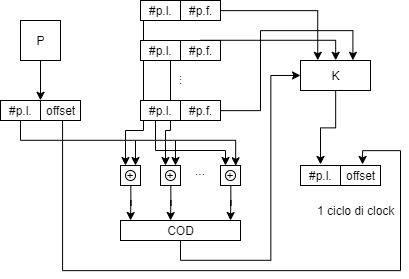
\includegraphics[scale=1]{mmu.png}
\end{center}
\subsection{Memoria Cache}
\begin{multicols}{2}
\begin{center}
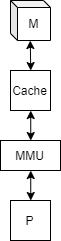
\includegraphics[scale=1]{memhierarchy.png}
\end{center}
Per rendere i calcolatori più veloci, quindi rendere l'accesso in memoria principale più rapido, usiamo delle \textbf{memorie cache} che sono \textbf{molto più piccole della memoria principale ma anche molto più veloci}.\\
L'idea è quella di \textbf{memorizzare nella cache} C \textbf{solo il working set} di un programma per rendere la traduzione degli indirizzi molto veloce.\\\\
dim(M) $>>$ dim (C)\\
t$_{aM}$ $>>$ t$_{aC}$\\
M = O(Gb), t$_a$ = O(100$\tau$)\\
C = O(Kb)/O(Mb\\\\
\textbf{Livelli di cache}\\
C$_2$ = 2--16 Mb, t$_a$ = O(10$\tau$)\\
C$_1$ = 16--32 Kb, t$_a$ = O(2--3$\tau$)
\end{multicols}
\pagebreak
Nella cache memorizziamo parole da 32 bit della memoria principale facenti parte del working set del processo in uso.
\begin{multicols}{2}
\begin{center}
\includegraphics[scale=0.9]{cacheline.png}
\end{center}
Quando il processo mi chiede di usare una parola non ancora caricata in cache, non solo viene memorizzata in cache tale parola ma anche le parole contigue che \textbf{probabilmente verranno usate negli istanti successivi} (principio di località).\\
Tale tecnica funziona poiché la memoria principale è una memoria interlacciata e mi consente in un solo ciclo di accedere a più indirizzi.
\end{multicols}
\subsection{Indirizzamento diretto}
\subsection{Indirizzamento completamente associativo}
\subsection{Indirizzamento associativo su insiemi}
\end{document}